% vim:et:ts=2:
% diese Datei enthaelt den eigentlichen Vortrag, siehe Handbuch zur Latex "Beamer" Klasse

\mode<presentation> {
  \usetheme{RWTHRZ}
}

\usepackage[german]{babel}
\usepackage[latin1]{inputenc}
\usepackage{times}
\usepackage[T1]{fontenc}
\usepackage[right]{eurosym}
\usepackage{graphicx}
\usepackage{hyperref}
\definecolor{darkblue}{rgb}{0,0,.5}
\hypersetup{pdftex=true, colorlinks=true, breaklinks=true, linkcolor=darkblue, menucolor=darkblue, pagecolor=darkblue, urlcolor=darkblue}

\title[Einf�hrung in git]{Einf�hrung in git}
\author[Gilger, Lederhofer]{}
\date[\today]{\today}

\begin{document}

\begin{frame}
  \begin{center}
  \vspace{1cm}
  \Huge Einf�hrung in git \\
  \vspace{1cm}
  
\includegraphics[scale=0.4]{img/git-logo.png} \\
  \vspace{0.6cm}
  \Large Johannes Gilger \& Matthias Lederhofer \\
  \small Rechen- und Kommunikationszentrum der RWTH Aachen \\
  \vspace{1cm}
  \small \today
  \end{center}
\end{frame}

\begin{frame}
  \frametitle{�bersicht}
  \begin{itemize}
    \item Begriffe in der Versionsverwaltung
    \item Unterschiede zentrale und dezentrale VCS
    \item Warum man git benutzen sollte
    \item Wie git funktioniert
    \item Wie wir git benutzen
    \item Weiterf�hrende Literatur und Software
  \end{itemize}
\end{frame}


\begin{frame}
  \frametitle{Begriffe}
  \begin{itemize}
    \item {\bf DVCS, VCS, SCM} - (Verteilte) Versionsverwaltung
    \item {\bf Repository} - Enth�lt die Geschichte (alle Versionen) eines Projekts
    \item {\bf Commit, Revision} - Identifiziert eine Version \\ SVN: 423, git: {\tt b8bba41...}
    \item {\bf Branch} - Ein Entwicklungszweig in der Geschichte
    \item {\bf Worktree} - Das aktuelle Arbeitsverzeichniss (Dateien)
    \item {\bf Checkout} - Die angelegten Dateien die einem bestimmten Stand entsprechen
  \end{itemize}
\end{frame}

\begin{frame}
  \frametitle{Zentrale Versionskontrolle ...}
  \begin{center}
    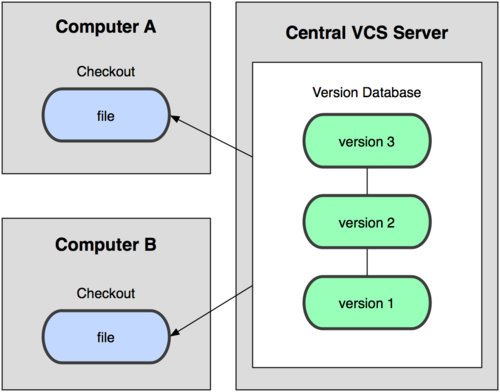
\includegraphics[width=8cm]{img/central_vcs.png}
  \end{center}
\end{frame}

\begin{frame}
  \frametitle{Dezentrale Versionskontrolle}
  \begin{center}
    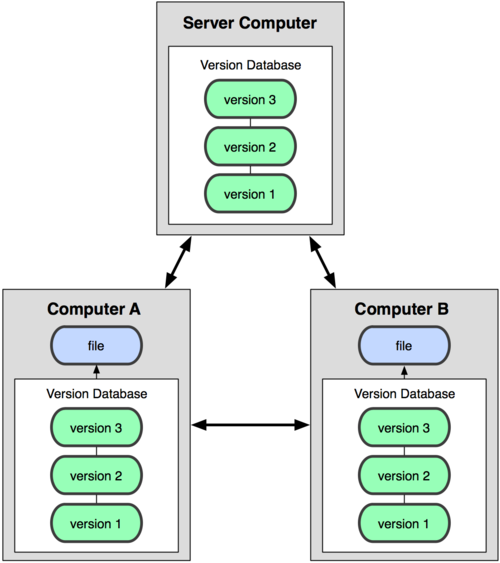
\includegraphics[width=6.3cm]{img/distributed_vcs.png}
  \end{center}
\end{frame}

\begin{frame}
  \frametitle{Typischer zentralisierter Workflow}
  \begin{center}
    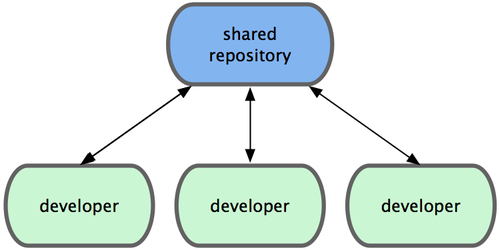
\includegraphics[width=9cm]{img/centralized_workflow.png}
  \end{center}
\end{frame}

\begin{frame}
  \frametitle{Typischer verteiler Workflow}
  \begin{center}
    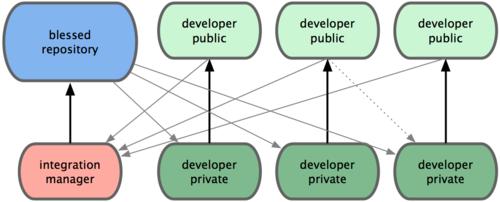
\includegraphics[width=10cm]{img/distributed_workflow.png}
  \end{center}
\end{frame}

\begin{frame}
  \frametitle{Kurze Geschichte von git}
  \begin{itemize}
    \item {\bf 2005:} Linus Torvalds schreibt git f�r die Entwicklung des Linux-Kernels \\ Anfangs sehr low-level und kompliziert
    \item {\bf 2005-2010:} Linus gibt die Entwicklung ab, schnell wachsende und aktive Community
    \item {\bf 2010:} git 1.7 ist aktuell, viele Open-Source Projekte sind inzwischen auf git umgestiegen \\ Android, Debian, Fedora, GIMP, Gnome, openSUSE, Perl, Ruby on Rails, VLC, Wine, X.org
    \end{itemize}
\end{frame}

\begin{frame}
  \frametitle{Warum sollte man git benutzen?}
  \begin{itemize}
    \pause
    \item Viele neue Konzepte, anfangs evtl.\ schwer zu verstehen \\ Ungef�hr einen Monat Einarbeitungszeit, zahlt sich jedoch schnell aus
    \pause
    \item ''SVN funktioniert doch / Viele Leute benutzen noch SVN'' \\ {\tt git-svn} hilft bei der Umstellung
    \pause
    \item ''Ich hab nicht vor Open-Source Software zu schreiben'' \\ git ist genauso hilfreich wenn man nur allein arbeitet
    \pause
    \item Andere Gr�nde?
  \end{itemize}
\end{frame}

\begin{frame}
  \frametitle{Vorteile von git gegen�ber SVN}
  \begin{itemize}
    \pause
    \item {\bf Geschwindigkeit} \\ git ist sehr schnell und speicherzeffizient, alle Operationen sind lokal (offline)
    \pause
    \item {\bf Kein Setup} \\ {\tt git init} und sofort loslegen, keine Erstellung von zentralen Projekten
    \pause
    \item {\bf Einfache Rechtevergabe} \\ Normale Dateisystemberechtigungen, Zugriff lokal oder z.B.\ �ber SSH
    \pause
    \item {\bf Schnelle parallele Entwicklung} \\ Keine Festlegung auf Regeln oder Rollen
  \end{itemize}
\end{frame}

\begin{frame}
  \frametitle{git Datenstrukturen und Dateilayout}
  \begin{block}{Die Datenstrukturen von git zu kennen...}
    \begin{itemize}
      \item Hilft enorm die Funktion der Befehle zu verstehen.
      \item Vermeidet falsche Arbeitsabl�ufe.
      \item Ist kein gro�er Aufwand.
    \end{itemize}
  \end{block}
\end{frame}

\begin{frame}
  \frametitle{Delta-Storage vs.\ Snapshots}
  \begin{center}
    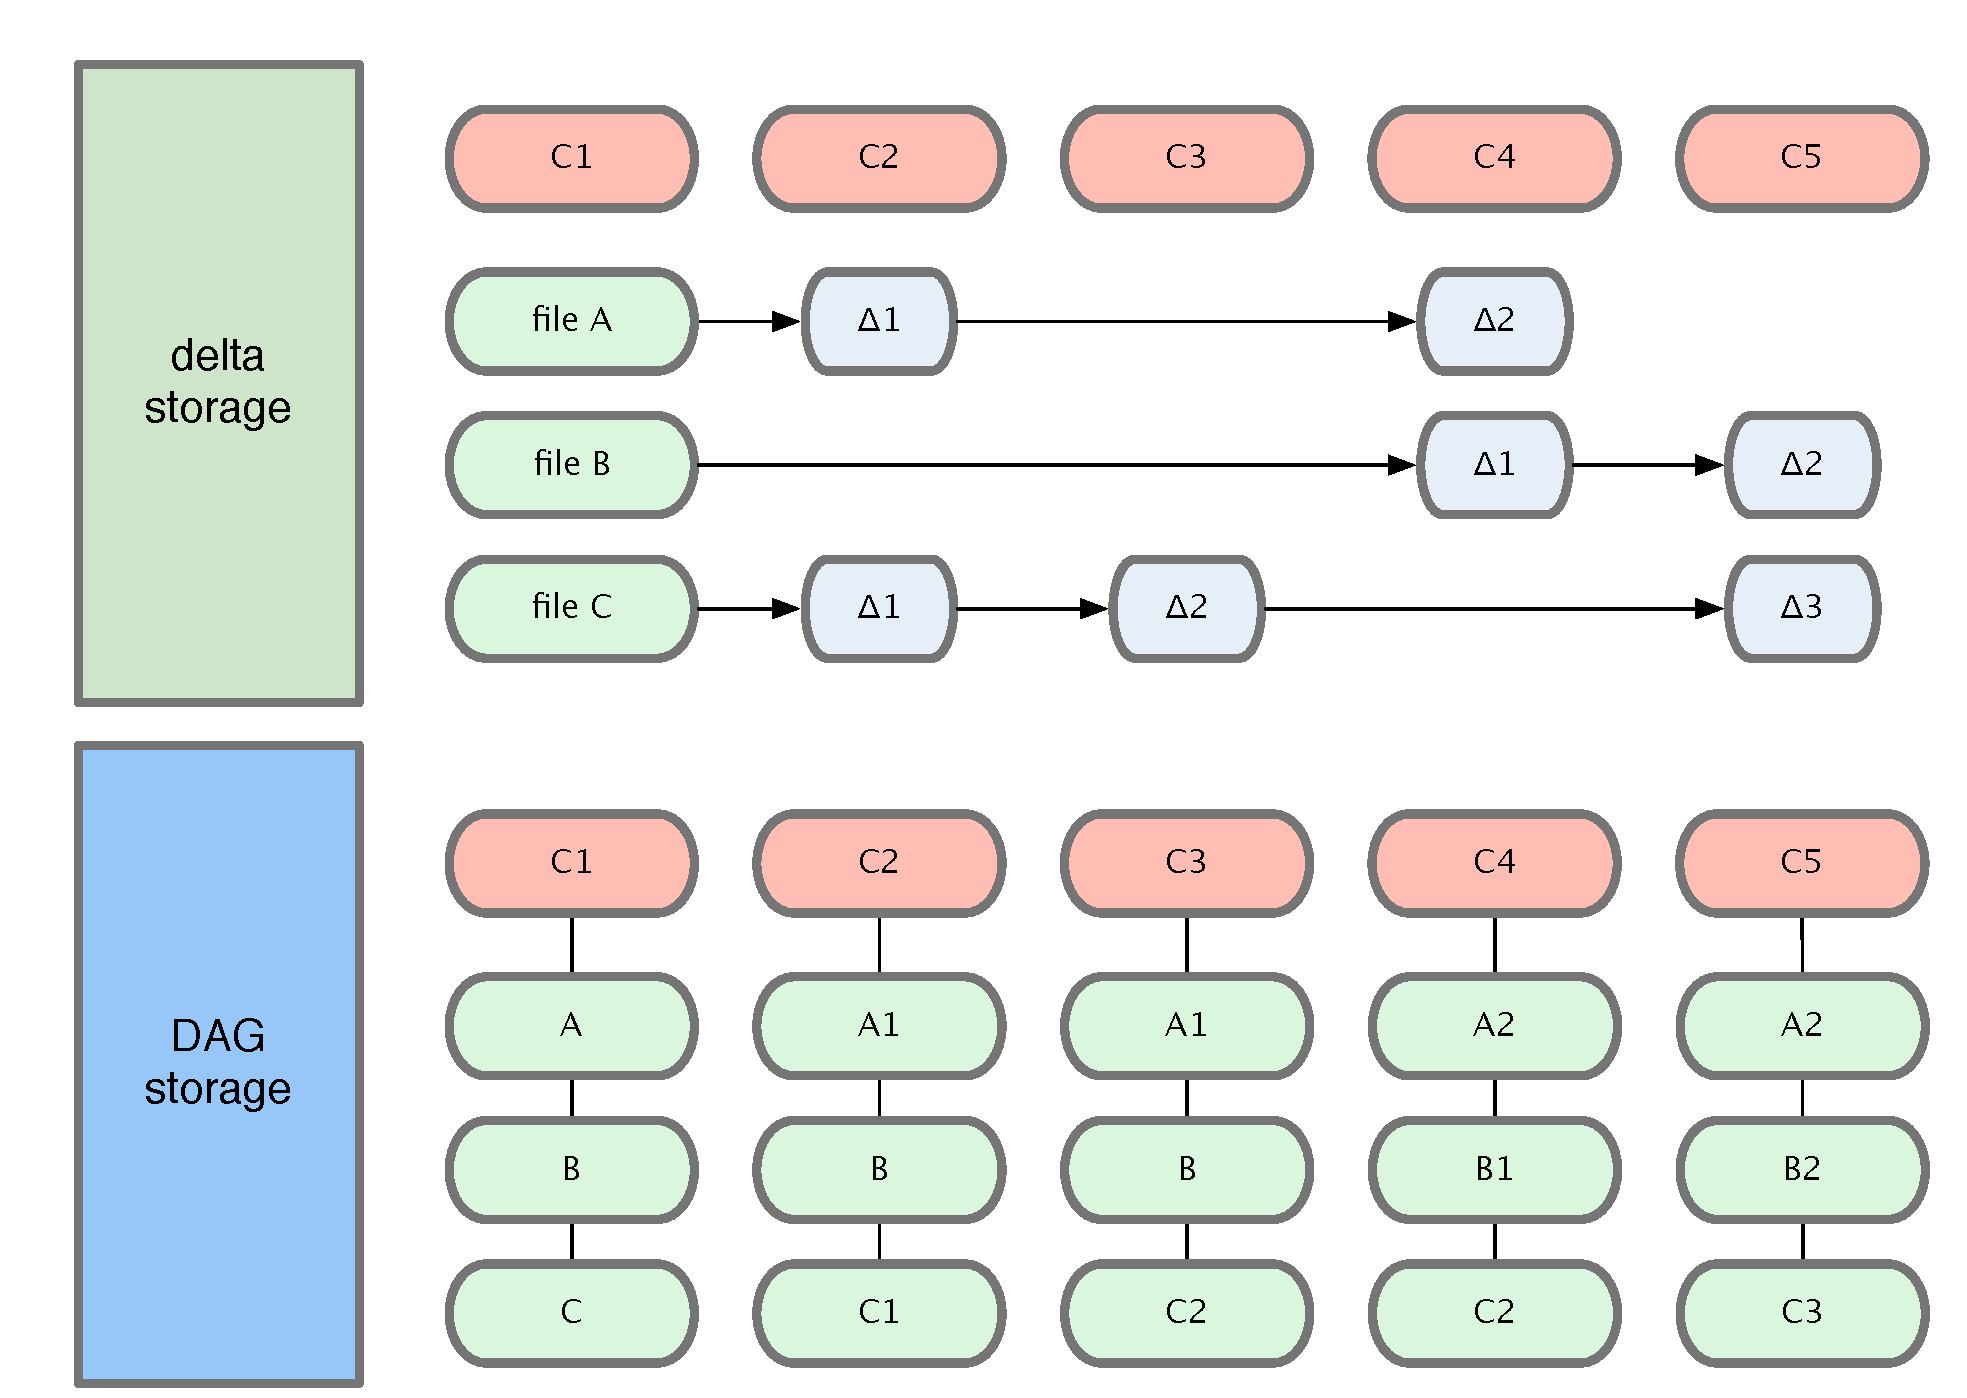
\includegraphics[width=9.5cm]{img/delta_storage.pdf}
  \end{center}
\end{frame}

\begin{frame}
  \frametitle{git ist ein Dateisystem mit Versionen}
  \begin{center}
    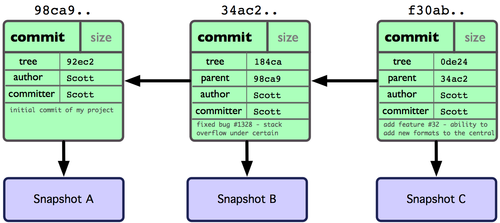
\includegraphics[width=9cm]{img/history_detailed.png} \\
    Wichtigstes Konzept: Die History ist eine einfach verlinkte Liste von Commits. Die Links zeigen ''zur�ck'', zeitlich gesehen.
  \end{center}
\end{frame}

\begin{frame}
  \frametitle{git ist eine Objekt-Datenbank}
  \begin{center}
    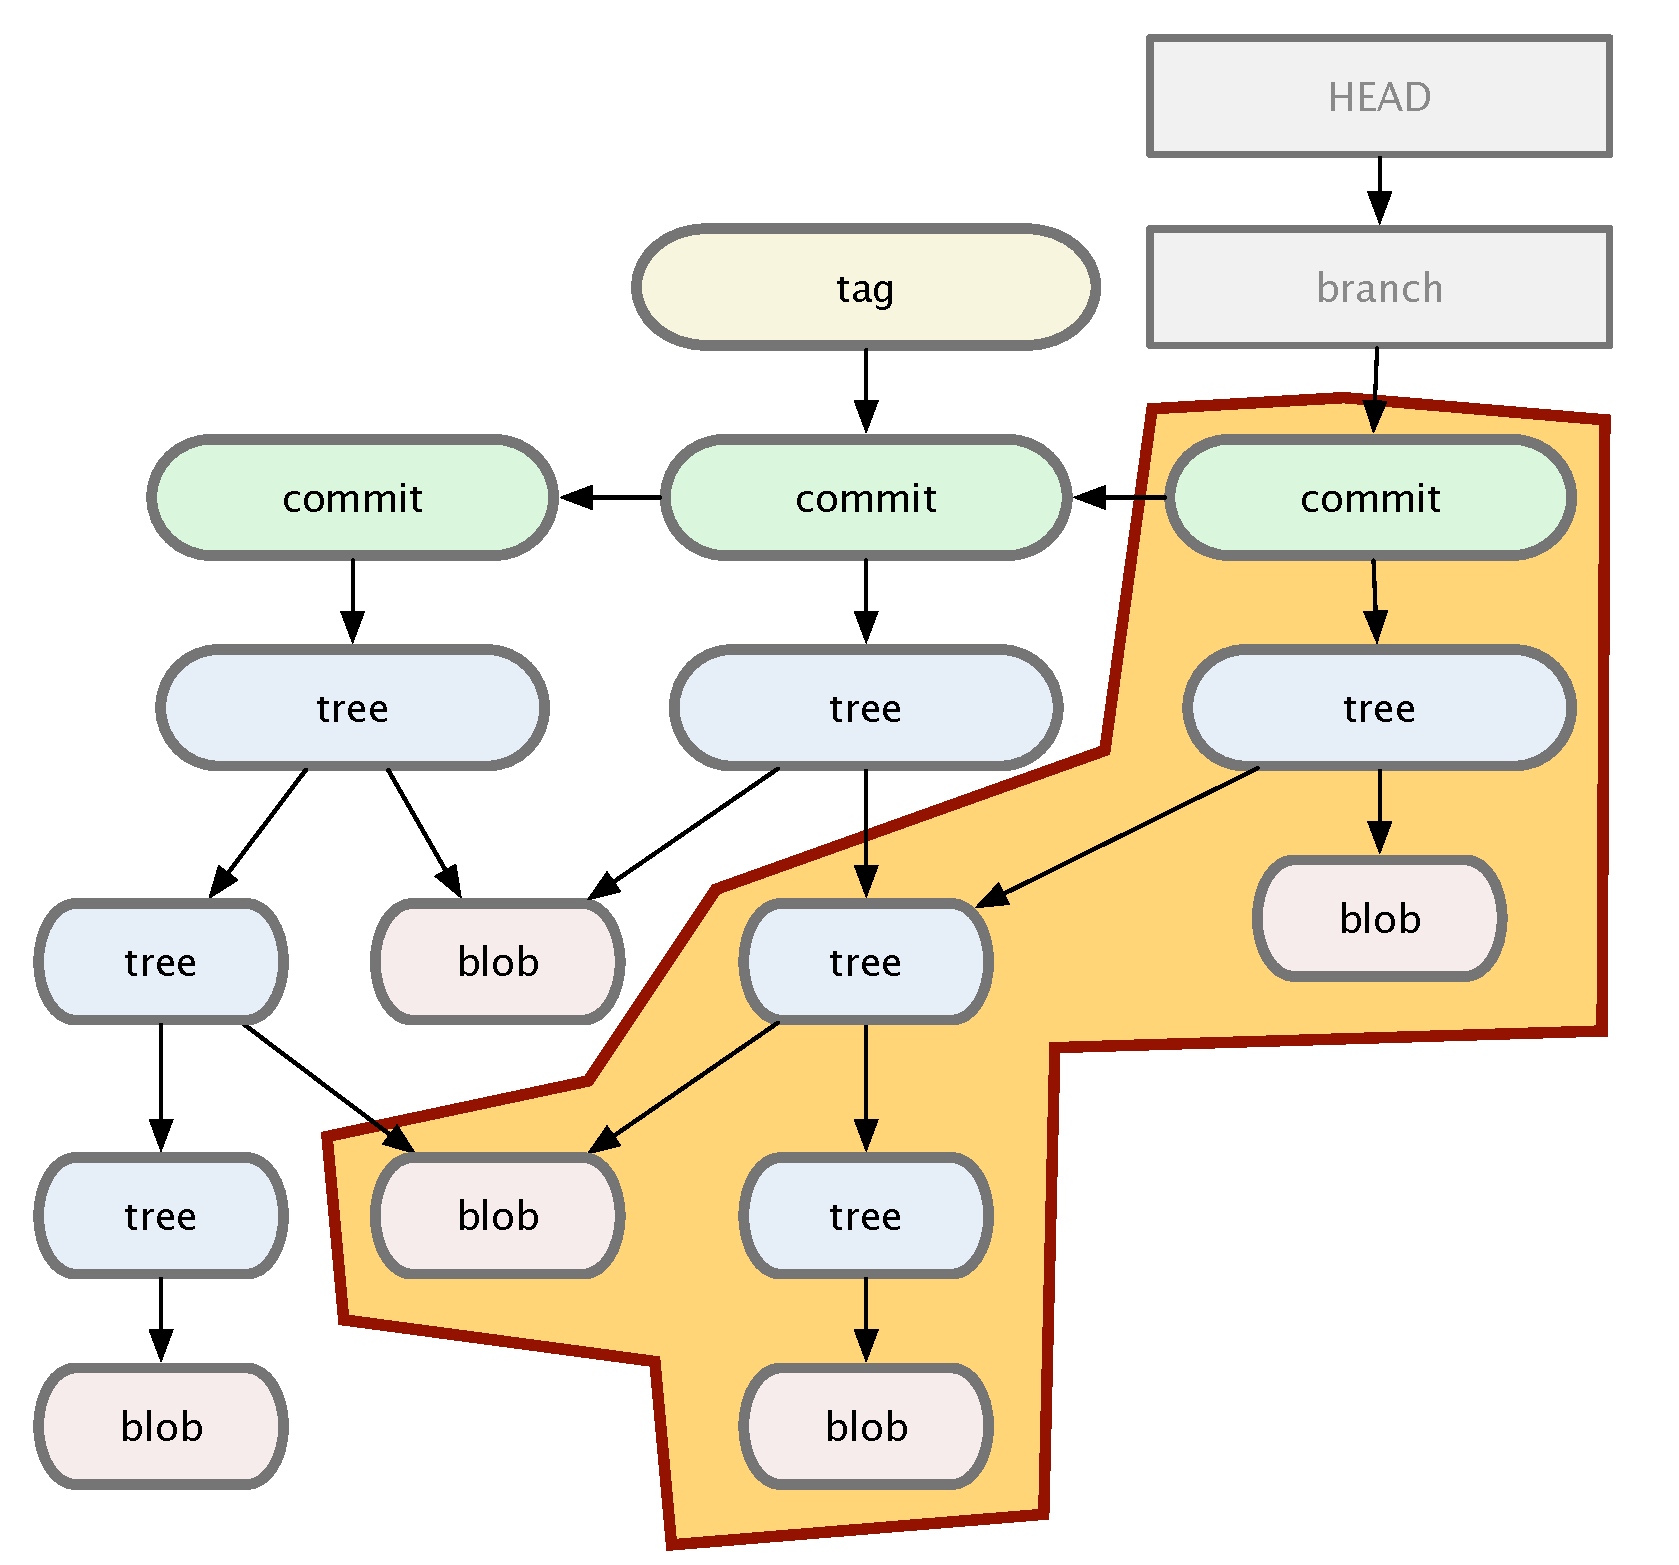
\includegraphics[width=7.8cm]{img/tree_commit.pdf}
  \end{center}
\end{frame}

\begin{frame}
  \frametitle{Commits und Branches}
  \begin{center}
    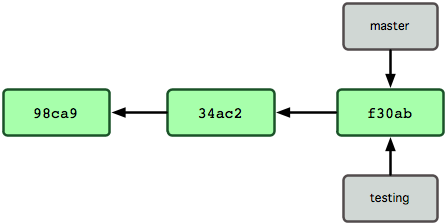
\includegraphics[width=10cm]{img/two_branches.png} \\
    Branches sind nur Zeiger (''references'') auf bestehende Commits
  \end{center}
\end{frame}

\begin{frame}
  \frametitle{HEAD - der aktuelle Branch}
  \begin{center}
    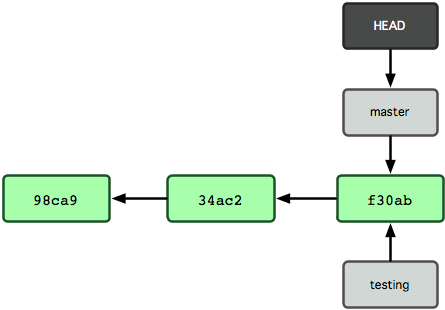
\includegraphics[width=8.5cm]{img/headref.png} \\
    HEAD zeigt an auf welchem Branch aktuell Commits gespeichert werden
  \end{center}
\end{frame}

\begin{frame}
  \frametitle{git checkout - den aktuellen Branch �ndern}
  \begin{center}
    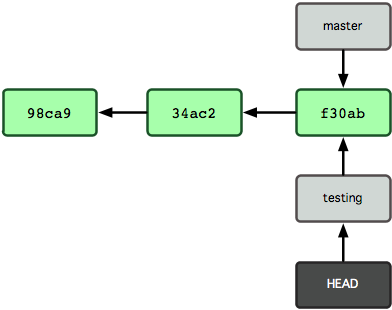
\includegraphics[width=8cm]{img/headref_changed.png} \\
    Ein Checkout aktualisiert den Worktree und den HEAD-Zeiger
  \end{center}
\end{frame}

\begin{frame}
  \frametitle{git commit - einen Commit erstellen}
  \begin{center}
    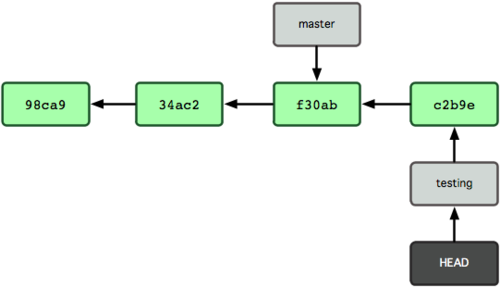
\includegraphics[width=10cm]{img/new_commit.png} \\
    Da HEAD auf ''testing'' zeigte wurde hier der Commit angelegt
  \end{center}
\end{frame}

\begin{frame}
  \frametitle{git checkout - zum ersten Branch zur�ck}
  \begin{center}
    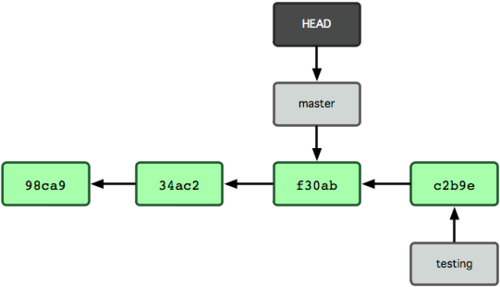
\includegraphics[width=10cm]{img/checkout.png} \\
    Es m�ssen w�hrenddessen noch �nderungen am Hauptentwicklungszweig vorgenommen werden
  \end{center}
\end{frame}

\begin{frame}
  \frametitle{git commit - ein paralleler Branch}
  \begin{center}
    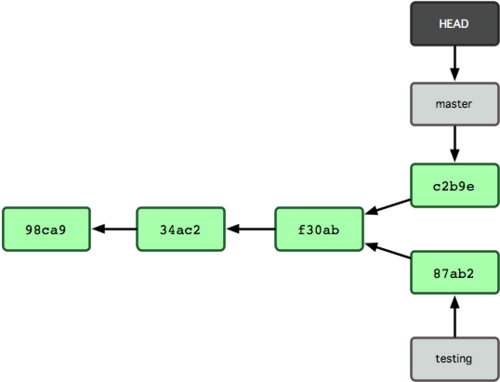
\includegraphics[width=9cm]{img/branch.png}
  \end{center}
\end{frame}

\begin{frame}
  \frametitle{Branching und Merging}
  \begin{center}
    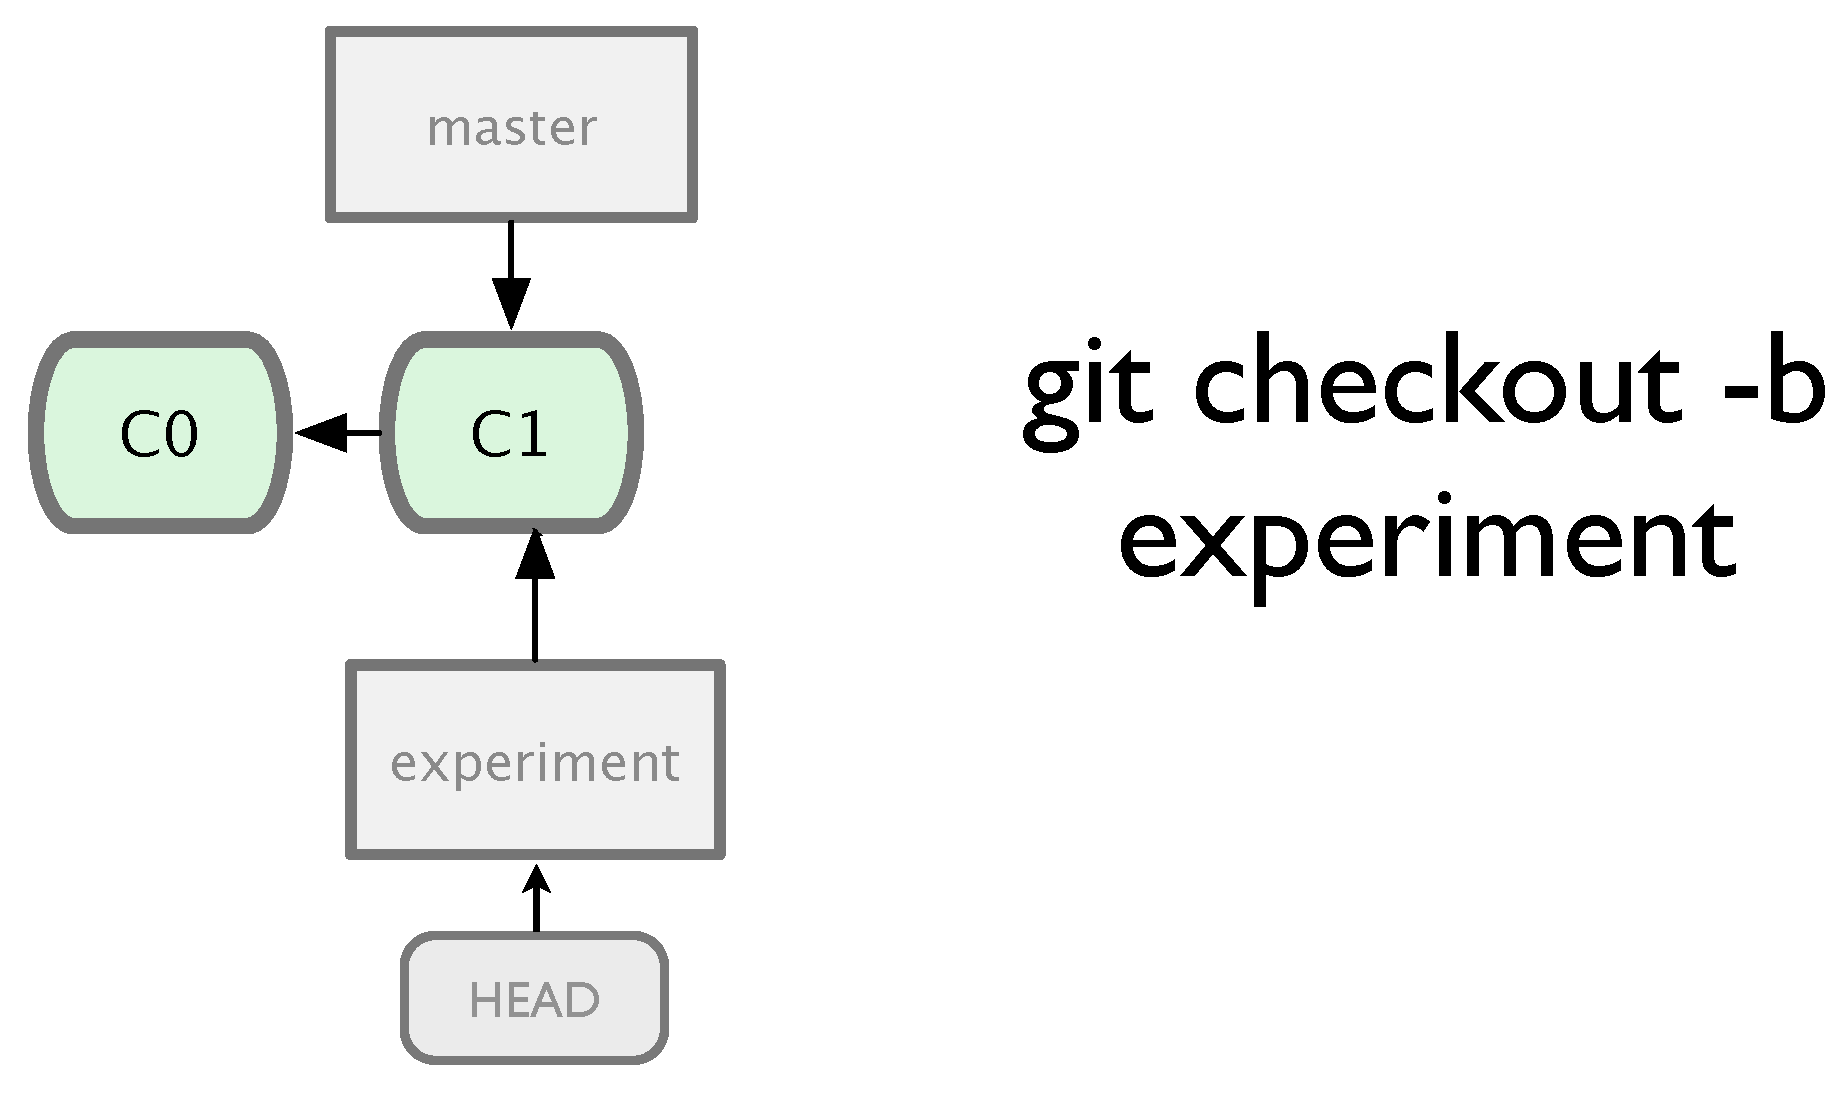
\includegraphics[width=9cm]{img/branch_1.pdf}
  \end{center}
\end{frame}

\begin{frame}
  \frametitle{Branching und Merging}
  \begin{center}
    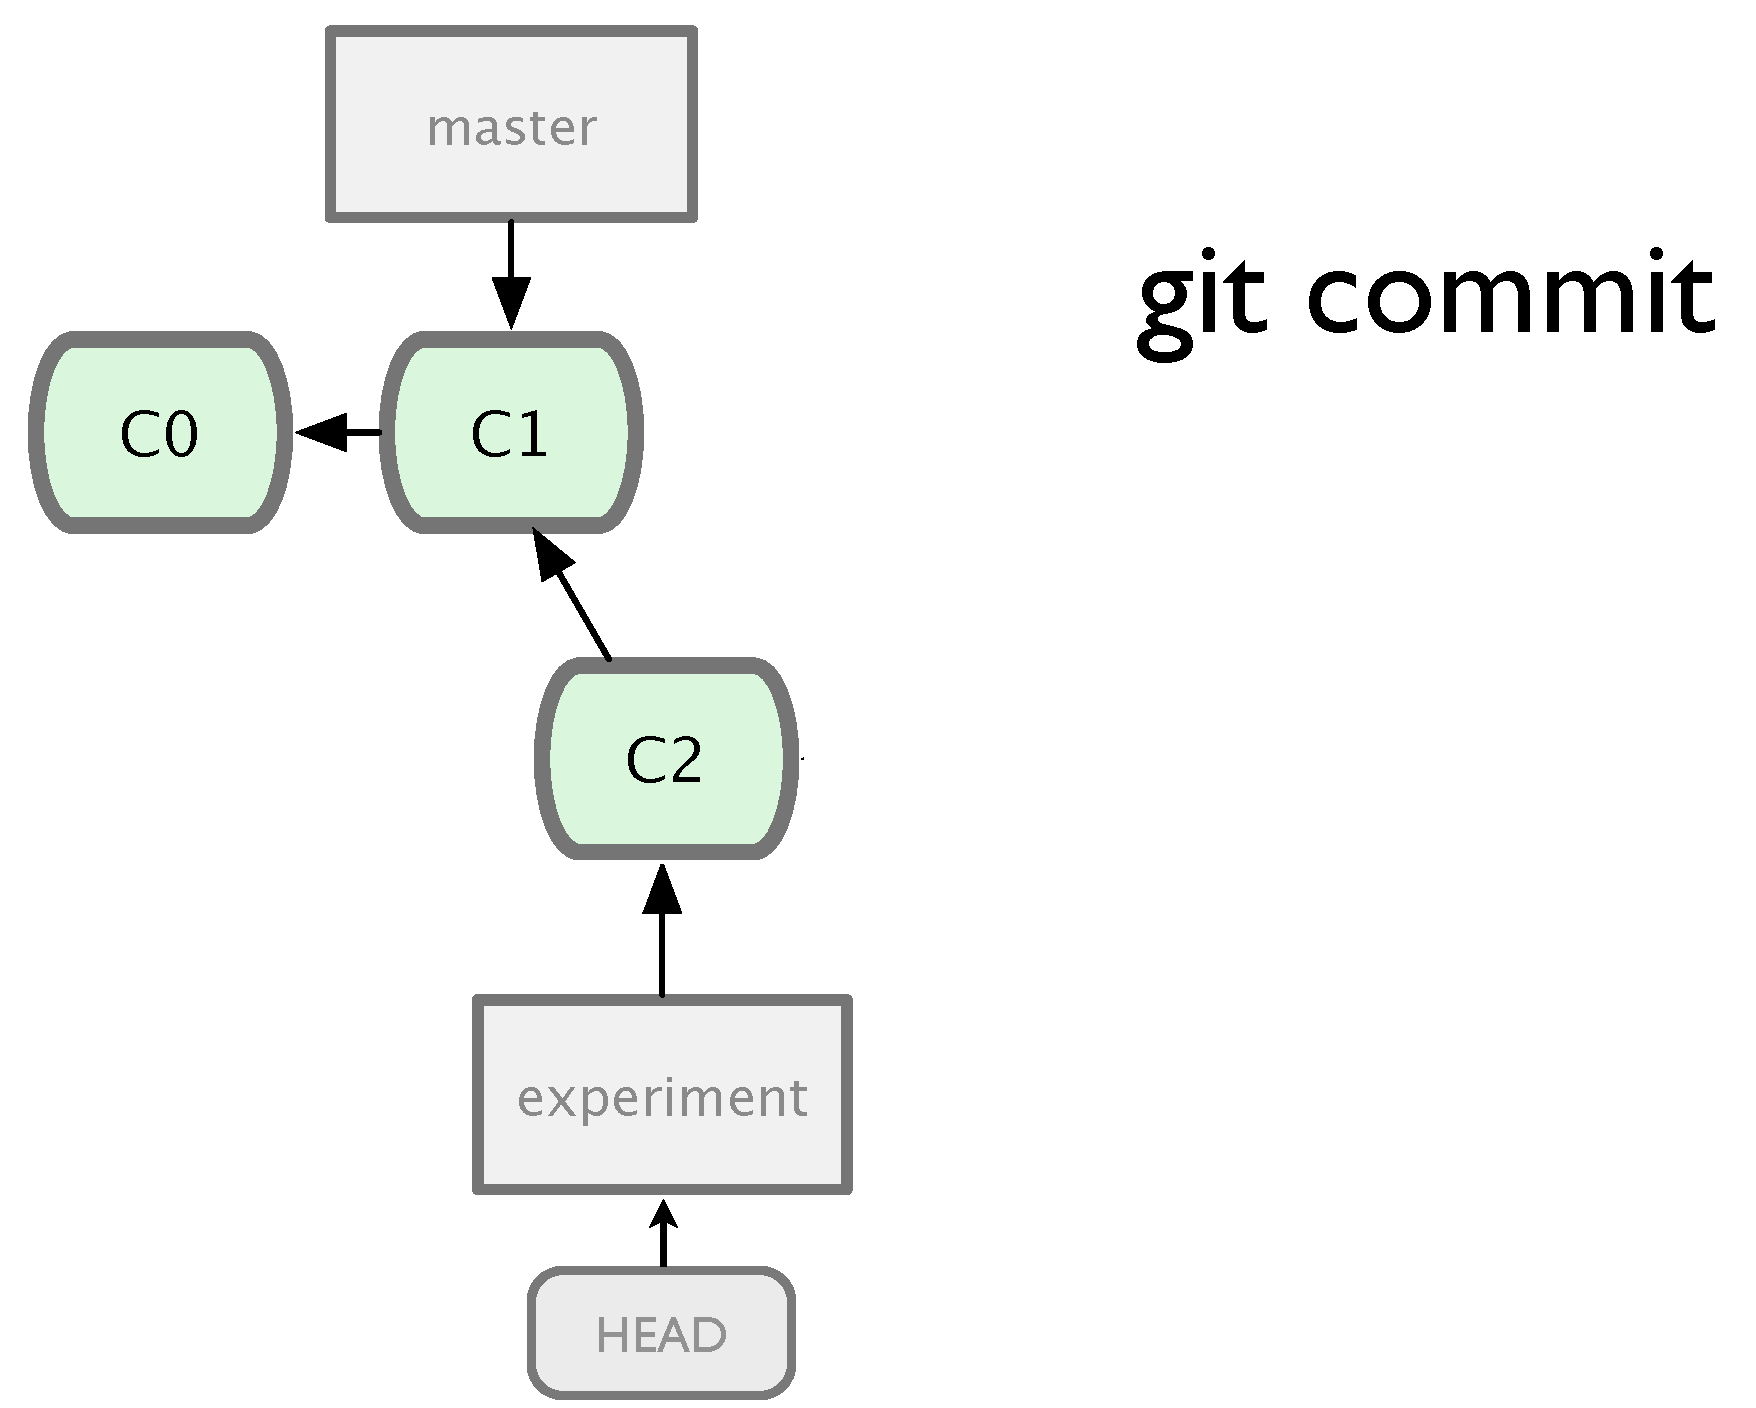
\includegraphics[width=9cm]{img/branch_2.pdf}
  \end{center}
\end{frame}

\begin{frame}
  \frametitle{Branching und Merging}
  \begin{center}
    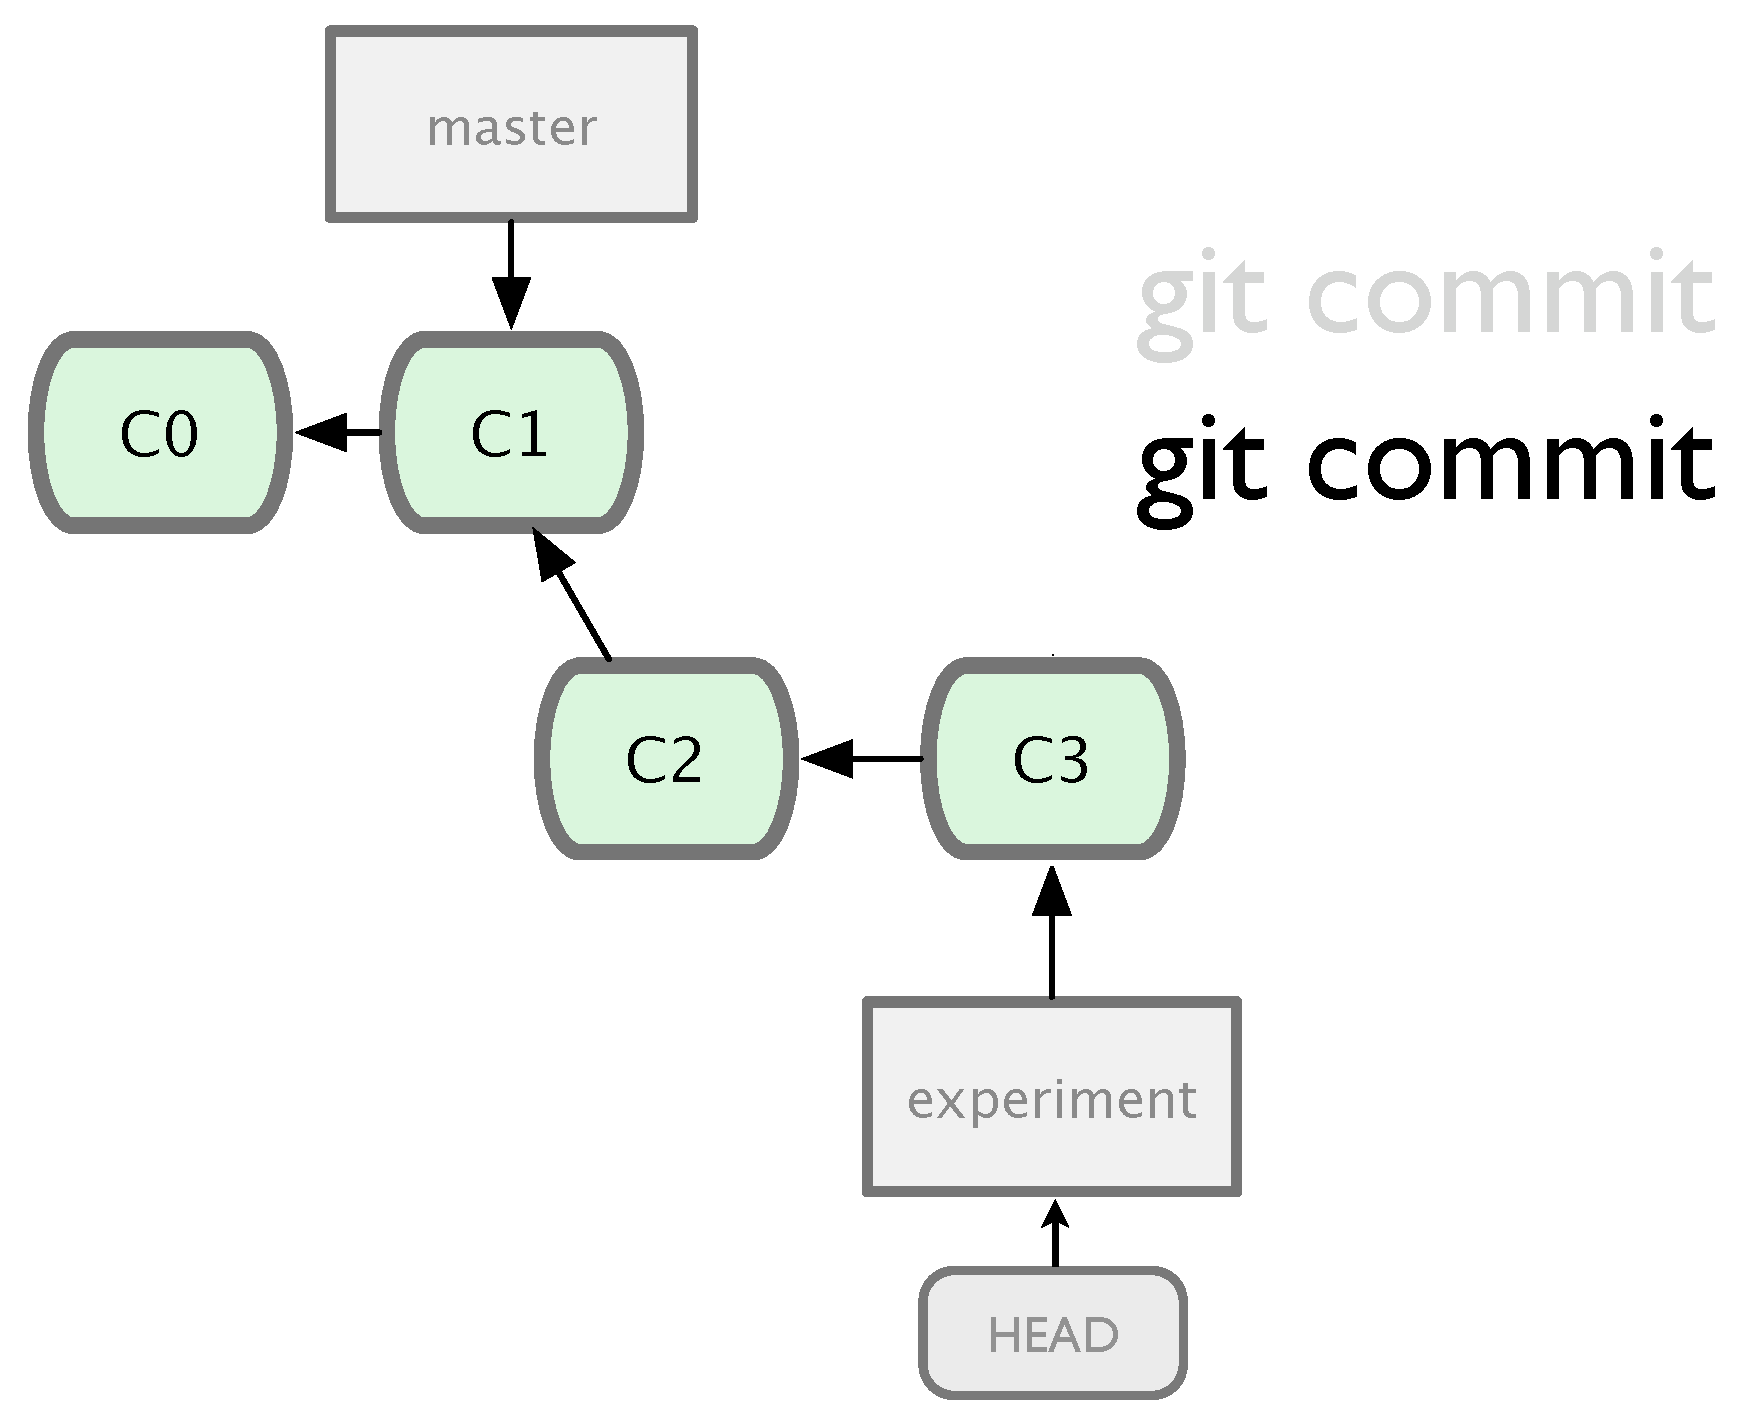
\includegraphics[width=9cm]{img/branch_3.pdf}
  \end{center}
\end{frame}

\begin{frame}
  \frametitle{Branching und Merging}
  \begin{center}
    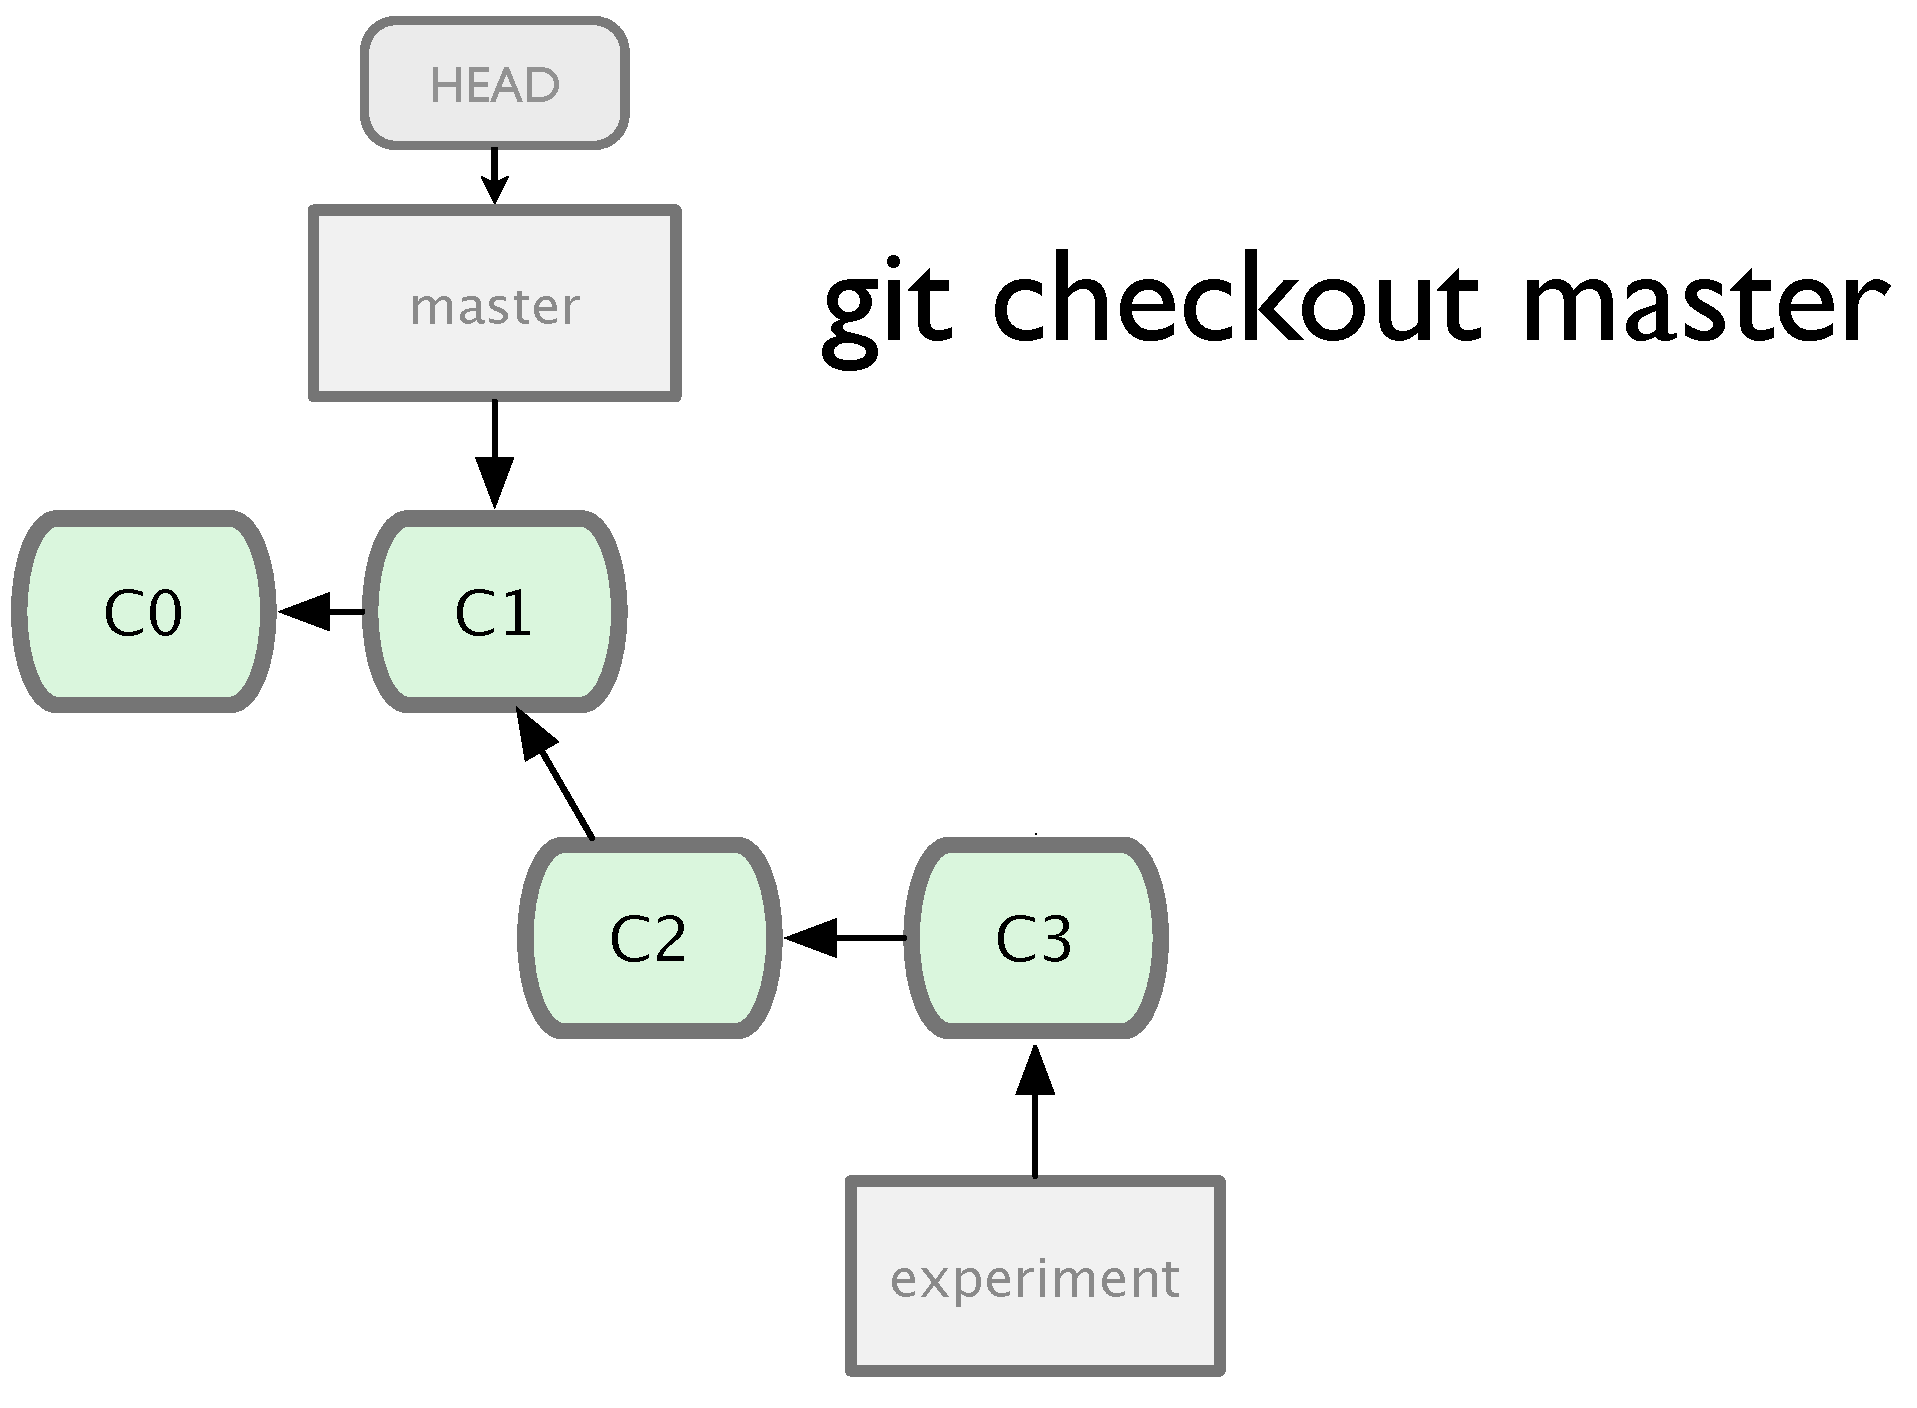
\includegraphics[width=9cm]{img/branch_4.pdf}
  \end{center}
\end{frame}

\begin{frame}
  \frametitle{Branching und Merging}
  \begin{center}
    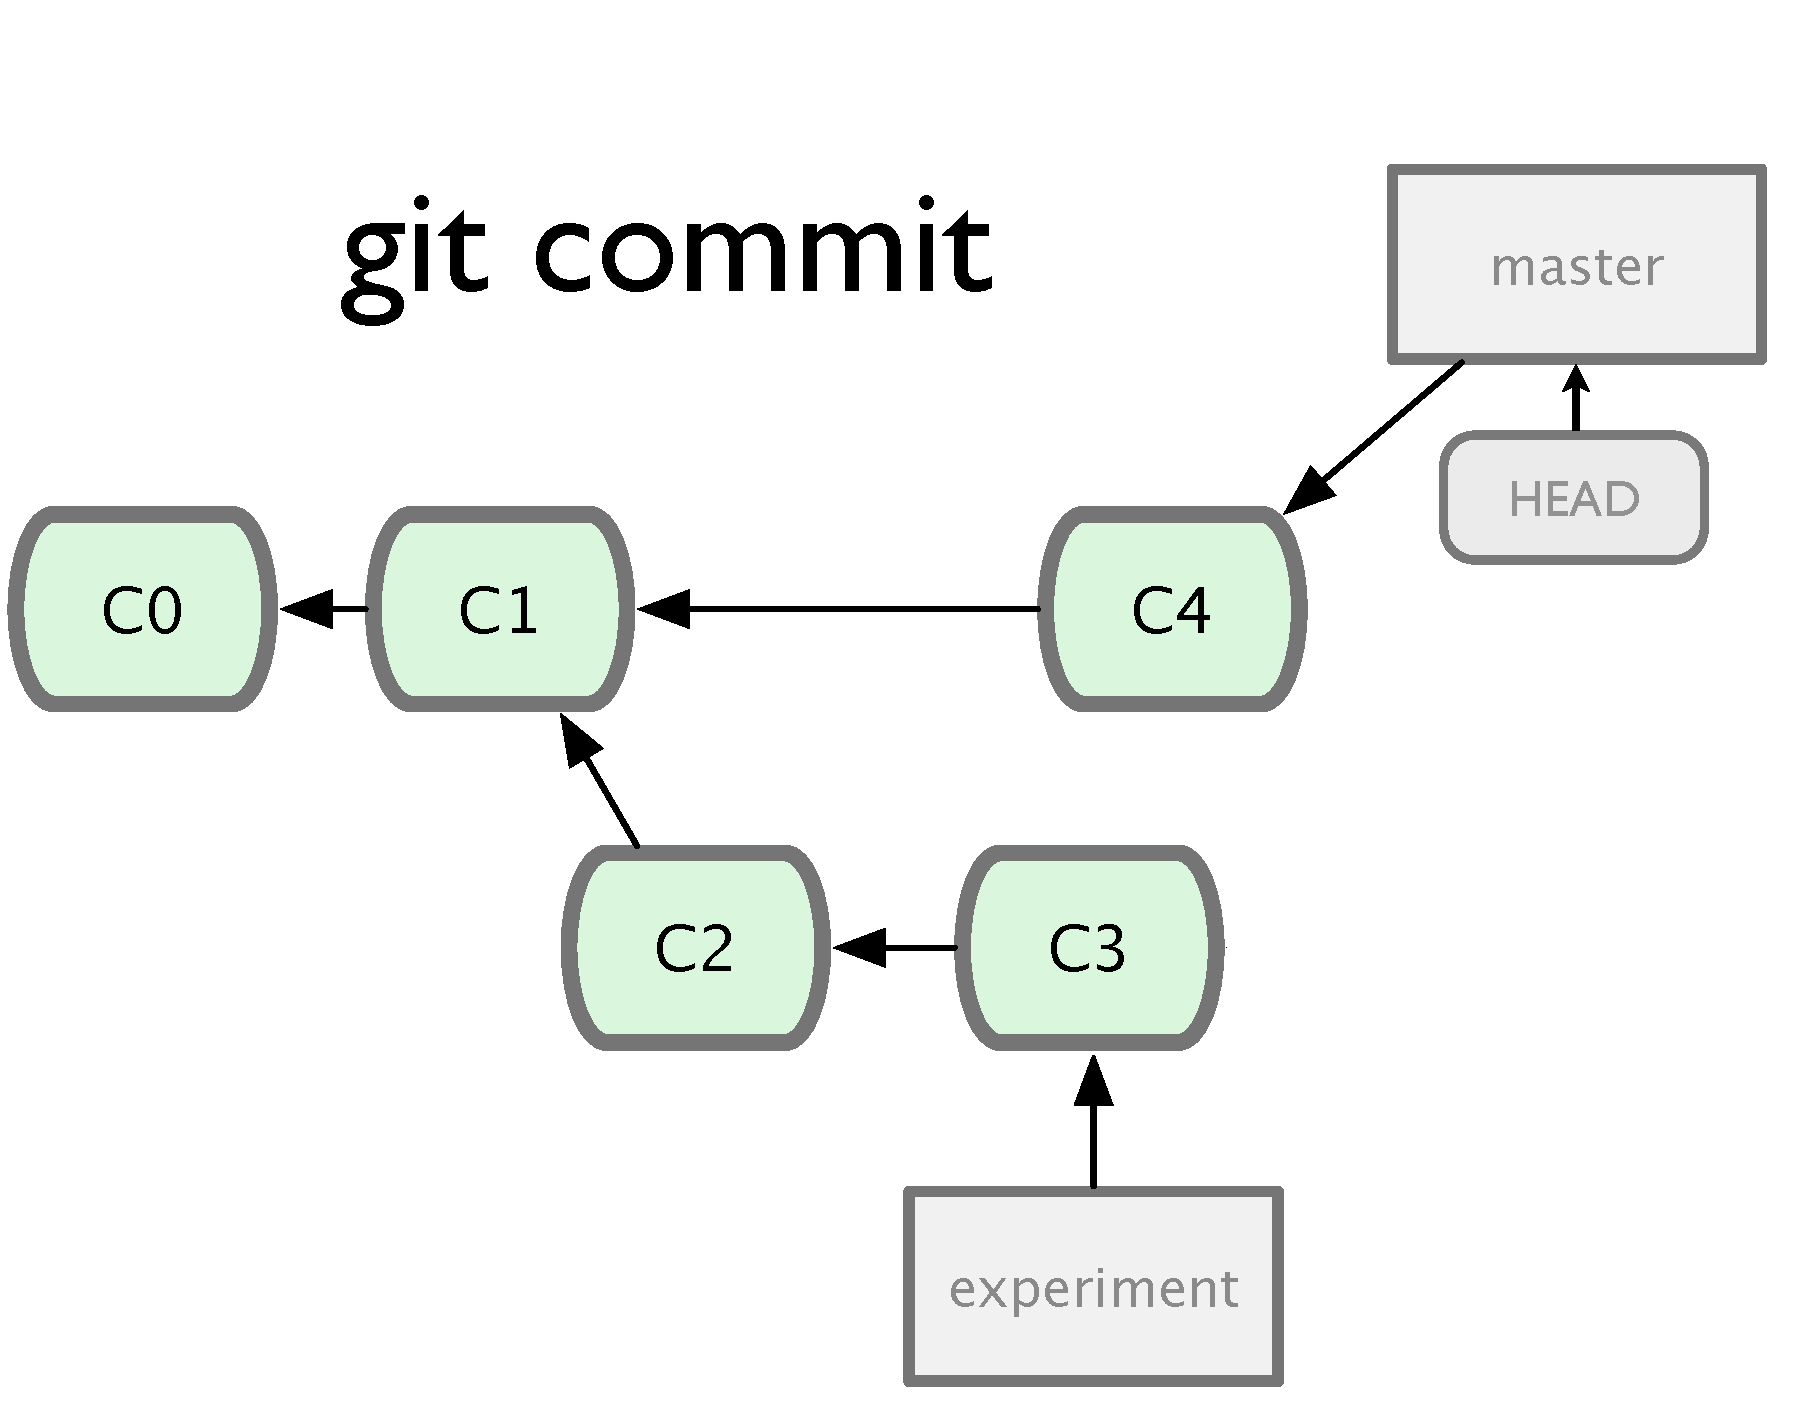
\includegraphics[width=9cm]{img/branch_5.pdf}
  \end{center}
\end{frame}

\begin{frame}
  \frametitle{Branching und Merging}
  \begin{center}
    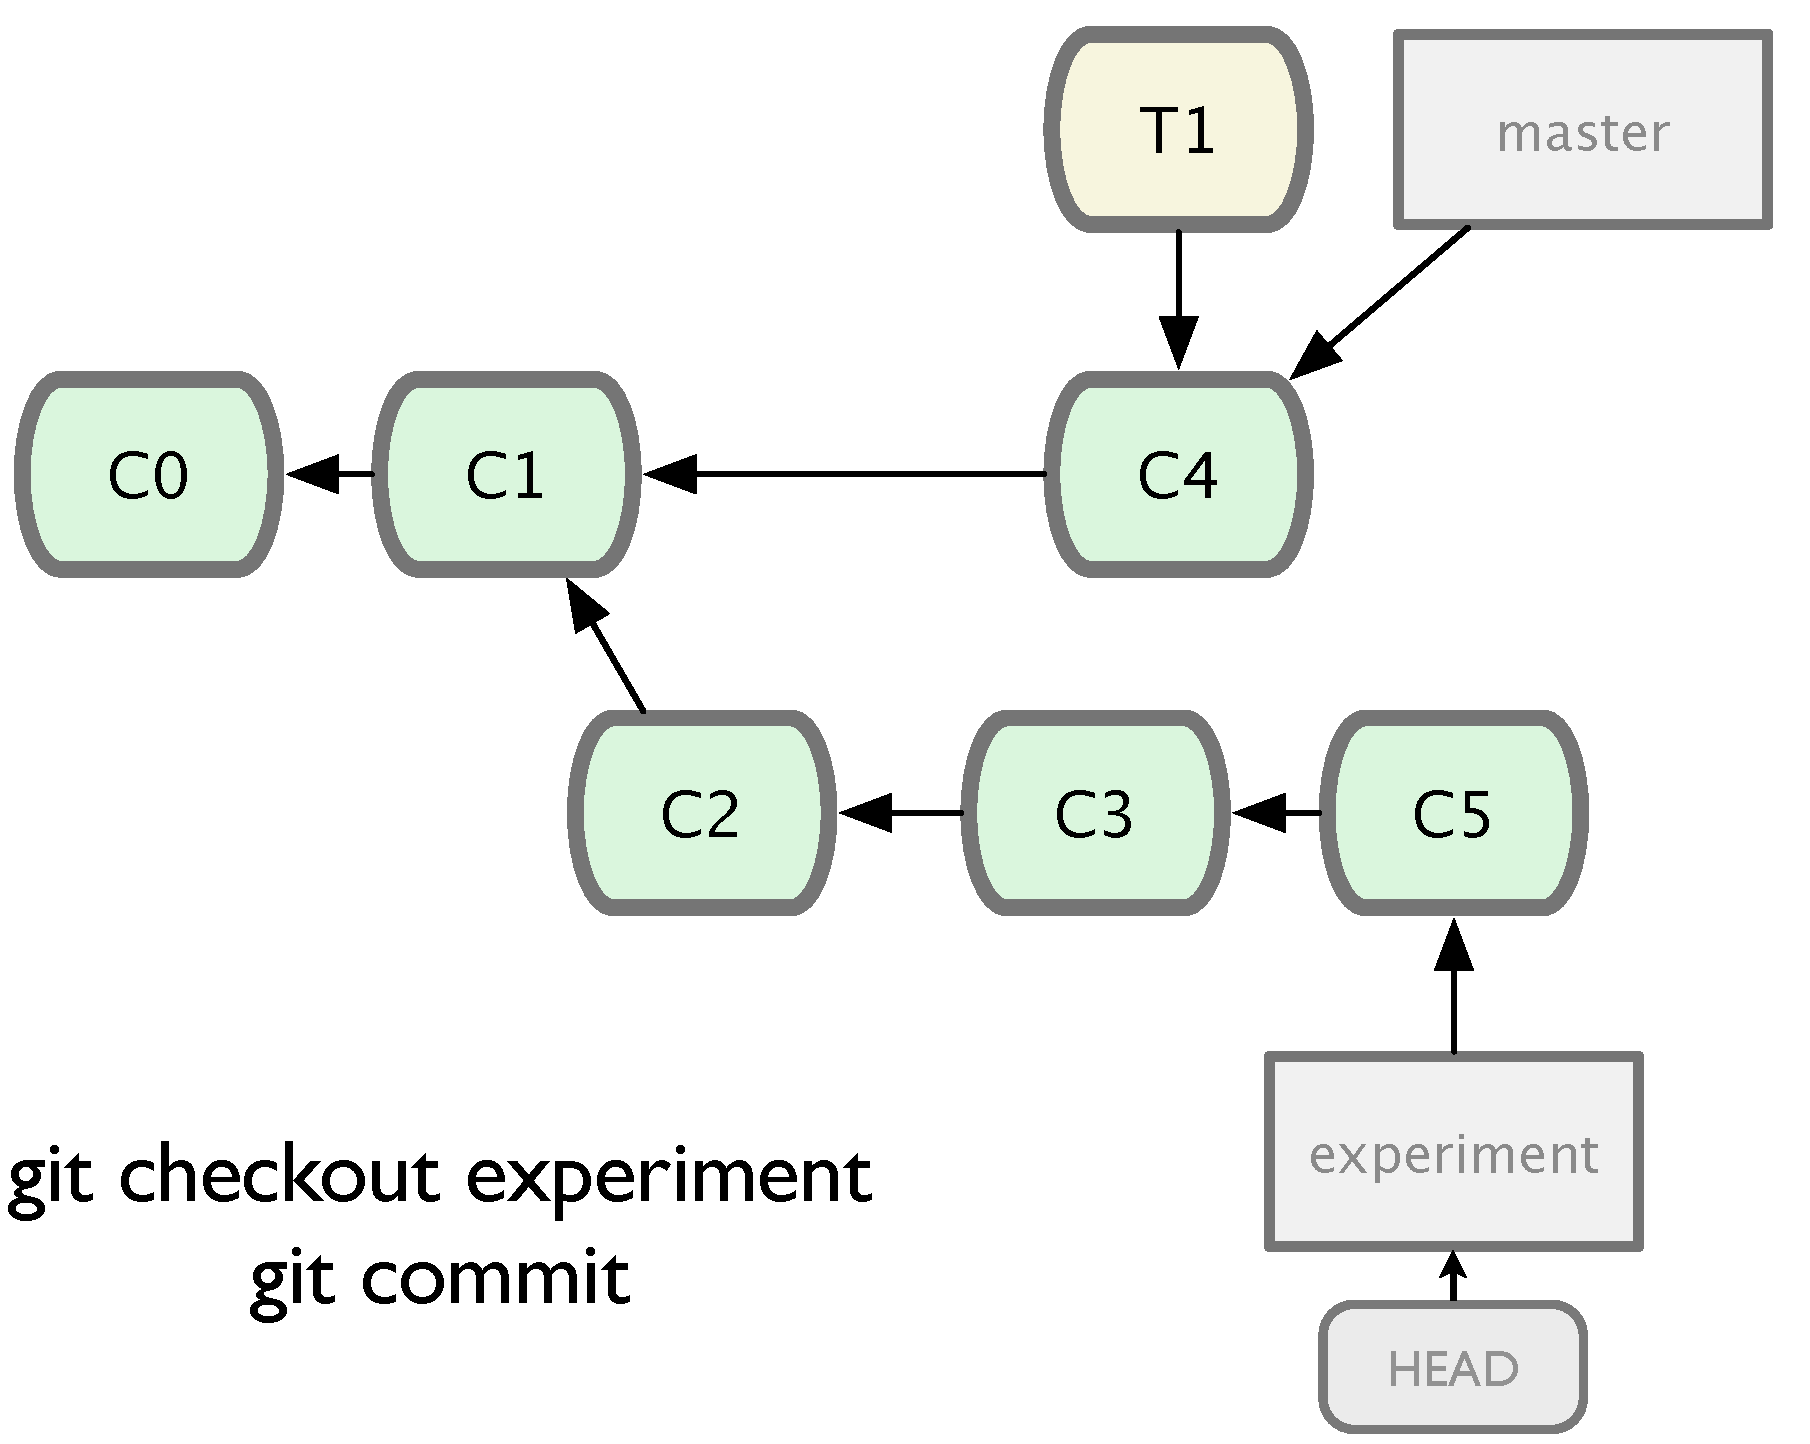
\includegraphics[width=9cm]{img/branch_6.pdf}
  \end{center}
\end{frame}

\begin{frame}
  \frametitle{Branching und Merging}
  \begin{center}
    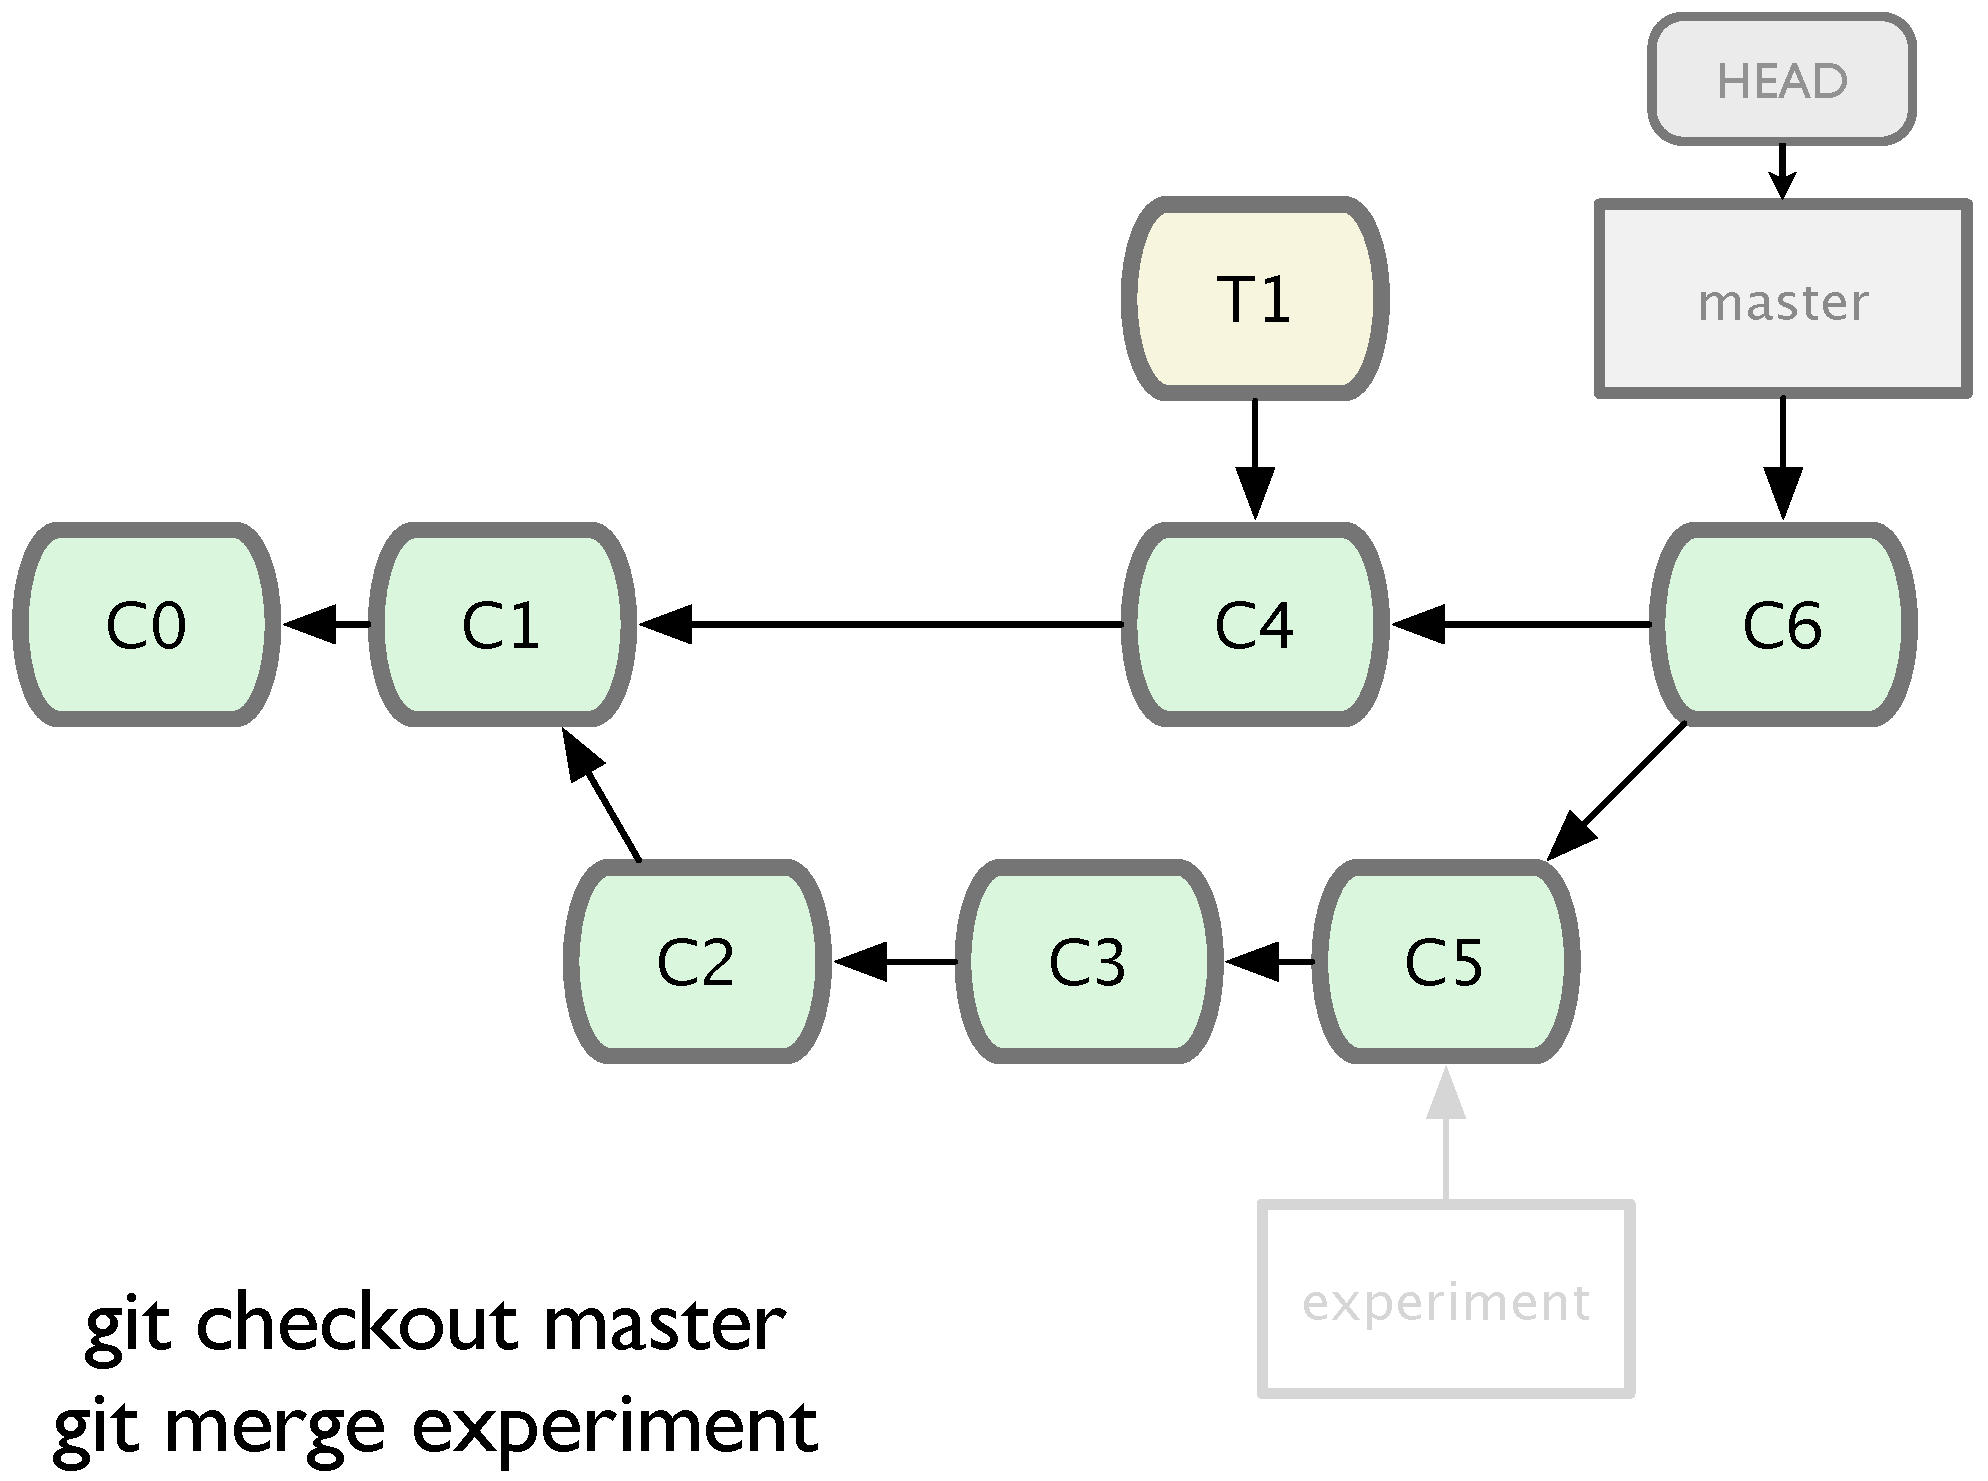
\includegraphics[width=9cm]{img/branch_7.pdf}
  \end{center}
\end{frame}

\begin{frame}
  \frametitle{Der Index / Stage}
  \vspace{-0.3cm}
  \begin{center}
    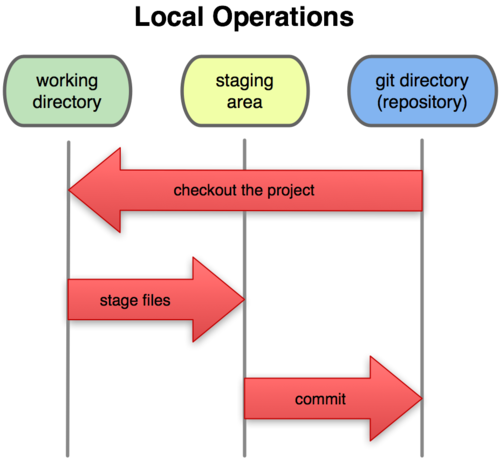
\includegraphics[width=7cm]{img/staging.png} \\
    Der Index ist ein sehr m�chtiges Konzept
  \end{center}
\end{frame}

\begin{frame}
  \frametitle{Der Index / Stage}
  \begin{center}
    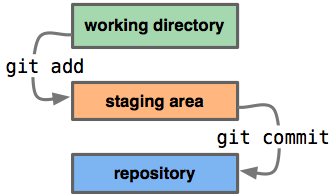
\includegraphics[width=5cm]{img/index1.png} \hspace{0.5cm} 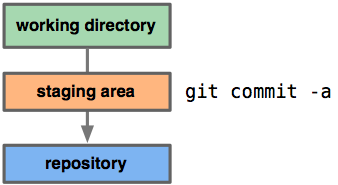
\includegraphics[width=5cm]{img/index2.png} \\
    Typische Arbeitsweise mit git (links). Workflow wie bei SVN (rechts) auch m�glich
  \end{center}
\end{frame}

\begin{frame}
  \frametitle{Dateizust�nde}
  \begin{center}
    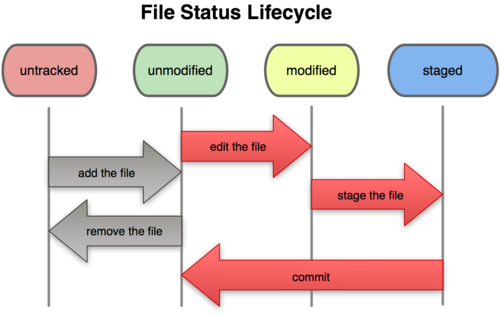
\includegraphics[width=10cm]{img/tracked.png}
  \end{center}
\end{frame}

\begin{frame}
  \frametitle{git revisions}
  \small F�r Befehle wie {\tt git log, git diff, git checkout, git show} etc.
  \begin{itemize}
    \item {\tt dae86e1950b1277e545cee180551750029cfe735 und dae86e} \\ SHA1 des Commits
    \item {\tt master} \\ Ein Branch (reference)
    \item {\tt master\~{}5} \\ Der f�nfte Vorg�nger des letzten Commits auf master
    \item {\tt master@\{yesterday\}} \\ Zustand von master gestern
  \end{itemize}
  Siehe auch {\tt git help rev-parse} f�r weitere Optionen
\end{frame}

\begin{frame}
  \frametitle{git revisions}
  \small F�r Befehle wie {\tt git log, git diff} etc.
  \begin{itemize}
    \item {\tt master..testing} \\ �nderungen in testing aber nicht in master
    \item {\tt master..} \\ �nderungen im aktuellen Branch die nicht in master sind
    \item {\tt ..master} \\ �nderungen die in master aber nicht im aktuellen Branch sind
    \item {\tt master...testing} \\ Symmetrische Differenz
  \end{itemize}
  Siehe auch {\tt git help rev-parse} f�r weitere Optionen
\end{frame}

\begin{frame}
  \frametitle{Wichtige git-Befehle - Arbeiten}
  \begin{itemize}
    \item {\tt git help <command>} \\ Hilfe zu git-commands, wichtigster Befehl ;)
    \item {\tt git init} \\ Ein git-Repo im aktuellen Verzeichniss beginnen
    \item {\tt git add} \\ Datei dem Index hinzuf�gen
    \item {\tt git status} \\ Status der Dateien im Arbeitsverzeichniss
    \item {\tt git diff} \\ Aktuelle �nderungen als diff anzeigen
    \item {\tt git commit} \\ Commit erstellen
  \end{itemize}
\end{frame}

\begin{frame}
  \frametitle{Wichtige git-Befehle - History}
  \begin{itemize}
    \item {\tt git log} \\ Log (History) anzeigen
    \item {\tt git branch} \\ Branches anzeigen (aktueller Branch hervorgehoben)
    \item {\tt git checkout <branch>} \\ Branch auschecken
    \item {\tt git show <object>} \\ Objekt (Branch, Commit, HEAD) anzeigen
    \item {\tt git blame -- <file>} \\ Anzeigen wer zuletzt welche Zeile ge�ndert hat
  \end{itemize}
\end{frame}

\begin{frame}
  \frametitle{Wichtige git-Befehle - Distribution und Branching}
  \begin{itemize}
    \item {\tt git branch -a} \\ Alle Branches anzeigen
    \item {\tt git pull} \\ Aktualisierung des Repositories vom Server
    \item {\tt git push} \\ Aktualisierung des Repositories auf den Server
    \item {\tt git merge <branch>} \\ Einbinden eines anderen Branches
    \item {\tt git remote} \\ Anzeigen von eingetragenen Servern
  \end{itemize}
\end{frame}

\begin{frame}
  \frametitle{Wichtige git-Dateien}
  \begin{itemize}
    \item {\tt \$HOME/.gitconfig} \\ git Benutzerkonfiguration 
    \item {\tt .gitignore} \\ Zum Ignorieren bestimmter Dateien bzw.\ Dateitypen, Verzeichnisweise und rekursiv
    \item {\tt .git} \\ git Repository, \emph{nur} im obersten Verzeichniss
    \item {\tt .git/config} \\ Konfiguration auf Repository-Ebene
    \item {\tt .git/objects} \\ Objektfiles bzw.\ Packfiles
    \item {\tt .git/refs} \\ Branches (References)
  \end{itemize}
\end{frame}

\begin{frame}
  \frametitle{Wichtige git-Dateien - Branches}
  Namespaces f�r refs (''references'') in {\tt .git}:
  \begin{itemize}
    \item {\tt .git/refs/heads} \\ Lokale Branches
    \item {\tt .git/refs/remotes} \\ Remote Branches
    \item {\tt .git/refs/tags} \\ Tags (Versionsnummern)
  \end{itemize}
  Das Arbeiten passiert \emph{immer} auf lokalen Branches, remote Branches werden nur von {\tt git pull} bzw.\ {\tt git fetch} ge�ndert.
\end{frame}

\begin{frame}
  \frametitle{git Tutorial}
  Initiale Konfiguration: \\
  {\tt \small git config $--$global user.name ''Johannes Gilger''} \\ 
  {\tt \small git config $--$global user.email ''gilger@rz.de''} \\

  Eventuell noch: \\
  {\tt \small git config $--$global color.ui ''auto''} \\ 
\end{frame}

\begin{frame}
  \frametitle{Das erste Repository}
  \vspace{-0.3cm}
  \begin{center}
    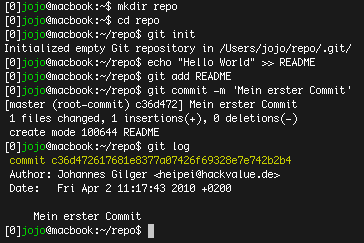
\includegraphics[width=8cm]{img/tutorial_1.png}
  \end{center}
\end{frame}

\begin{frame}
  \frametitle{Das erste Repository}
  \vspace{-0.3cm}
  \begin{center}
    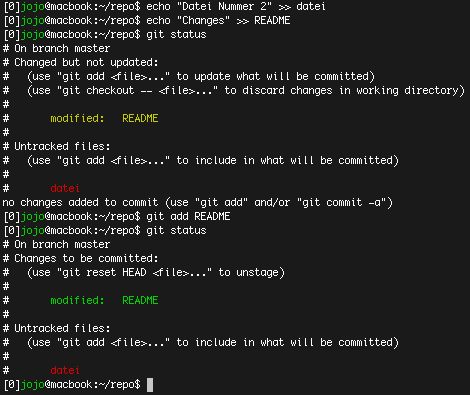
\includegraphics[width=8cm]{img/tutorial_2.png}
  \end{center}
\end{frame}

\begin{frame}
  \frametitle{Das erste Repository}
  \vspace{-0.3cm}
  \begin{center}
    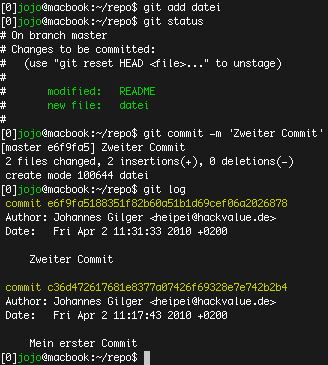
\includegraphics[width=6cm]{img/tutorial_3.png}
  \end{center}
\end{frame}

\begin{frame}
  \frametitle{git Installation \& Interfaces}
  \begin{itemize}
    \item {\bf Linux:} Installation mittels Distribution \\ Grafische Programme: {\tt gitk} und {\tt git gui}
    \item {\bf Mac OS X:} Installation mittels fink / MacPorts oder git-osx-installer \\ Grafische Programme: {\tt gitk} oder \href{http://gitx.frim.nl/}{GitX}
    \item {\bf Windows:} Installation per \href{http://code.google.com/p/msysgit/}{msysgit} \\ Grafische Programme: \href{http://code.google.com/p/tortoisegit/}{tortoisegit}
  \end{itemize}
  $\Rightarrow$ Wie immer ist die \href{http://git-scm.com}{git-Webseite} der beste Anlaufpunkt

\end{frame}

\begin{frame}
  \frametitle{git GUIs - GitX}
  \vspace{-0.3cm}
  \begin{center}
    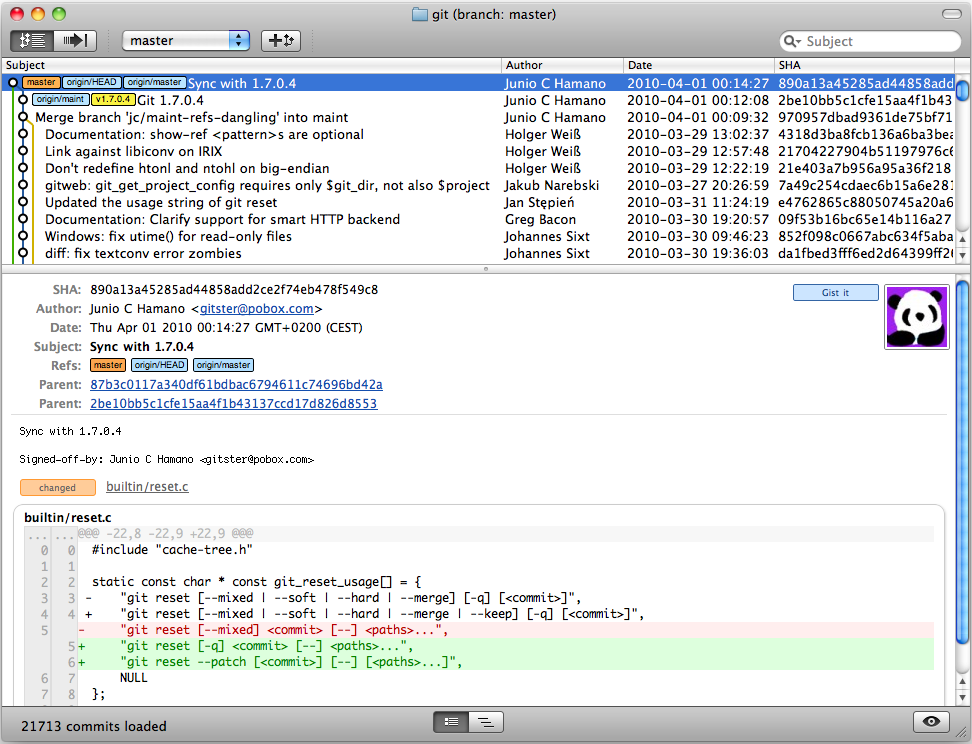
\includegraphics[width=9.5cm]{img/gitx.png}
  \end{center}
\end{frame}

\begin{frame}
  \frametitle{git GUIs - gitk}
  \vspace{-0.3cm}
  \begin{center}
    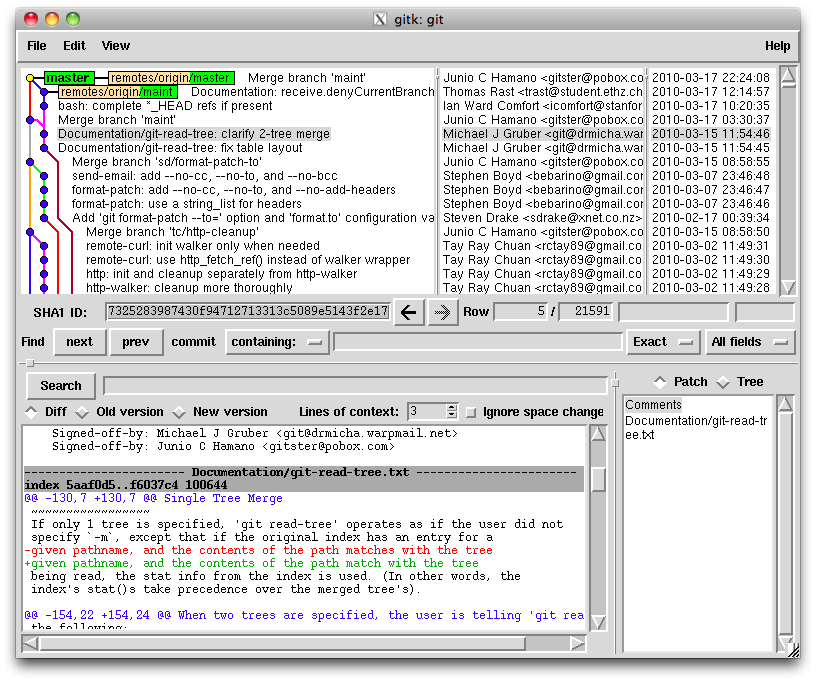
\includegraphics[width=9.0cm]{img/gitk.png}
  \end{center}
\end{frame}

\begin{frame}
  \frametitle{git GUIs - git gui}
  \vspace{-0.3cm}
  \begin{center}
    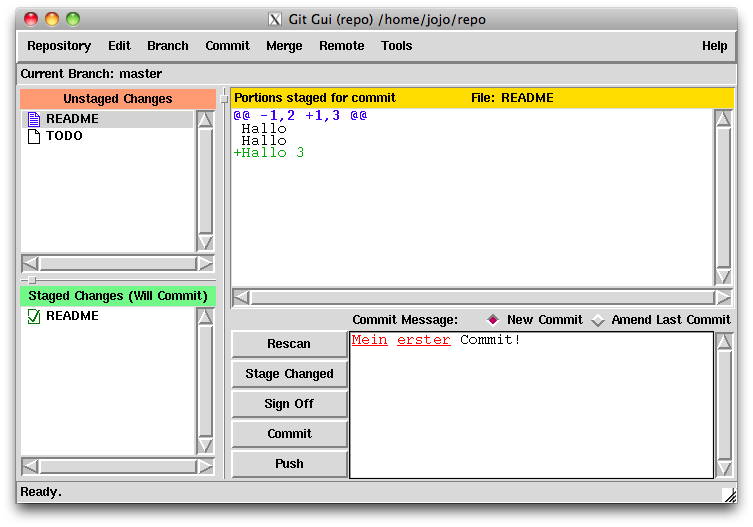
\includegraphics[width=9.5cm]{img/git_gui.png} \\
    Dateien k�nnen abschnittsweise committed werden
  \end{center}
\end{frame}

\begin{frame}
  \frametitle{git GUIs - tortoisegit}
  \vspace{-0.3cm}
  \begin{center}
    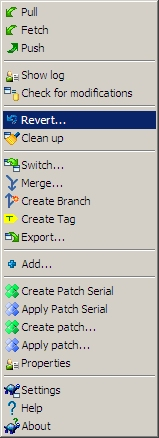
\includegraphics[width=2.5cm]{img/tortoisegit.png}
  \end{center}
\end{frame}

\begin{frame}
  \frametitle{git GUIs - tortoisegit}
  \vspace{-0.3cm}
  \begin{center}
    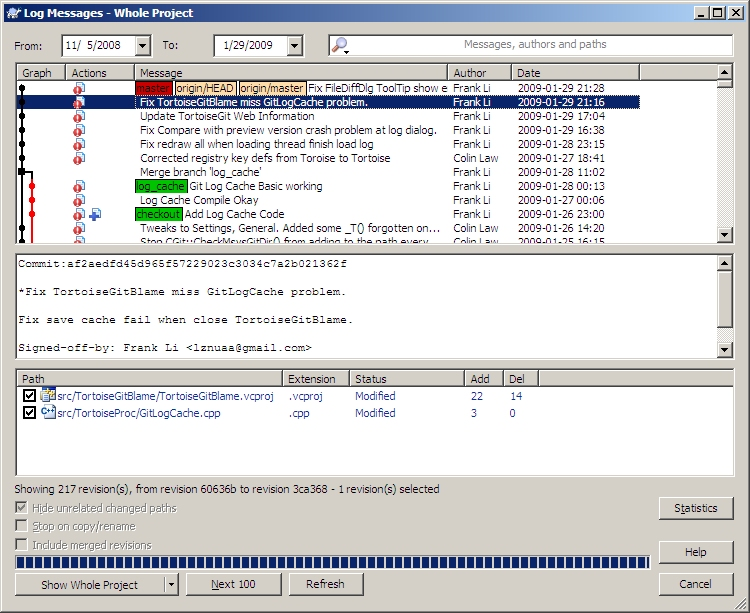
\includegraphics[width=9cm]{img/tortoisegit2.png}
  \end{center}
\end{frame}

\begin{frame}
  \frametitle{Wie wir im NOC git benutzen}
  \begin{itemize}
    \item {\bf Szenario 1:} Entwicklung (kleinerer) Webanwendungen \\ Meistens an Ort und Stelle (.git), sehr schnell und einfach
    \item {\bf Szenario 2:} �nderung an externer Software festhalten \\ (z.B.\ wenn Software von uns ''shibbolized'' wird)
    \item {\bf Szenario 3:} Gr��ere Projekte mit mehreren Mitarbeitern. Ausgezeichnete Versionen (v0.5) direkt unterst�tzt
  \end{itemize}
\end{frame}

\begin{frame}
  \frametitle{Wie wir im NOC git benutzen}
  \vspace{-0.8cm}
  \begin{center}
    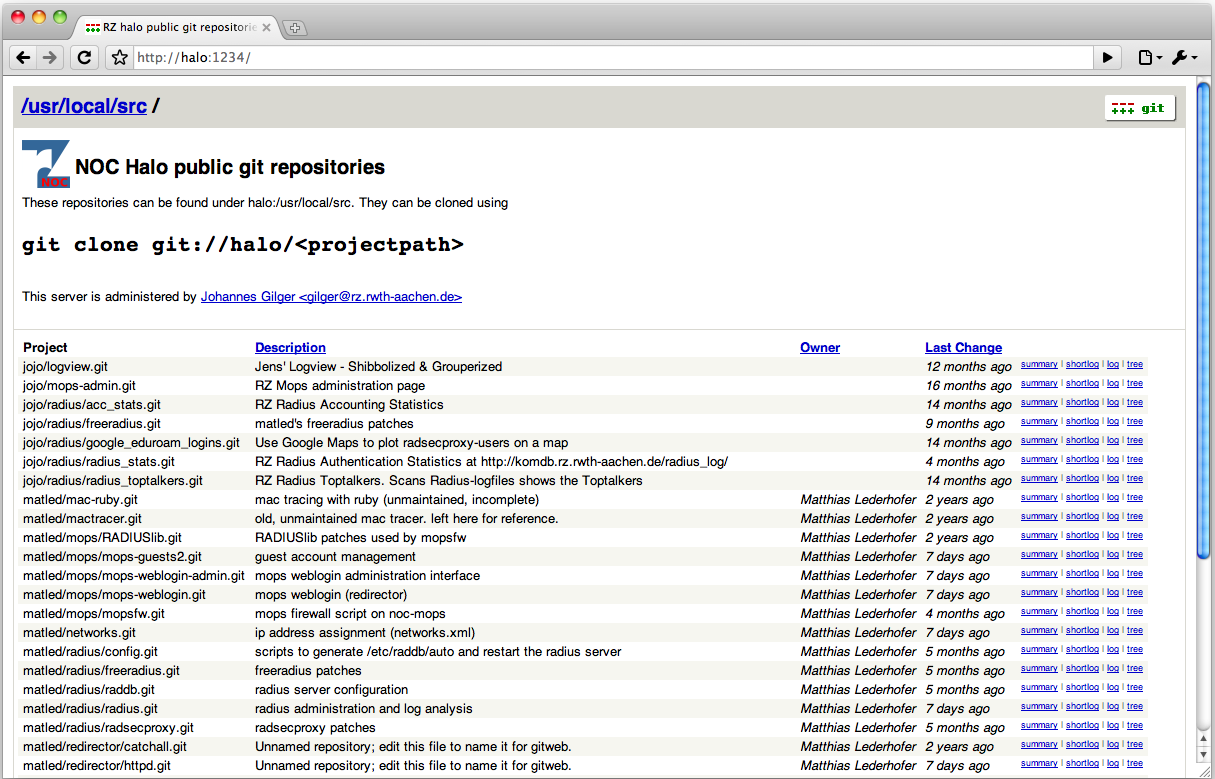
\includegraphics[width=11cm]{img/git_halo.png}
  \end{center}
\end{frame}

\begin{frame}
  \frametitle{Wie wir im NOC git benutzen}
  \vspace{-0.3cm}
  \begin{center}
    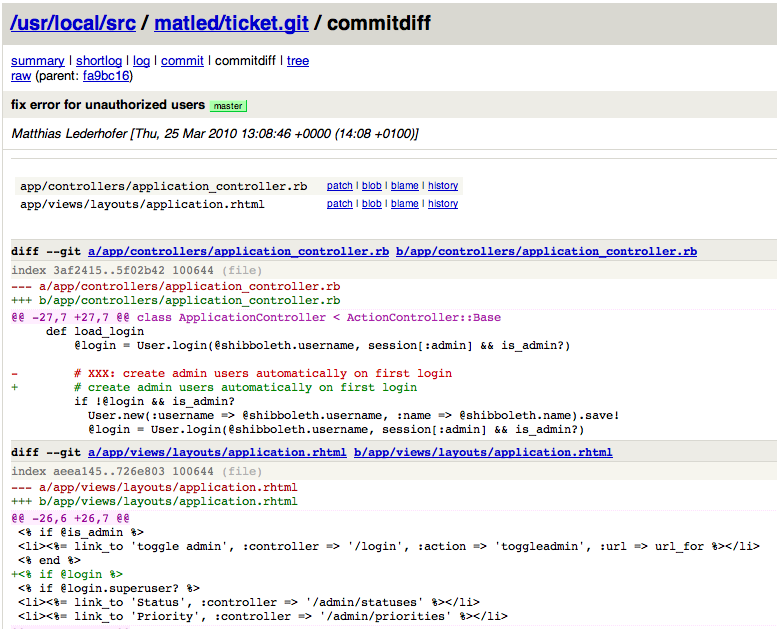
\includegraphics[width=9cm]{img/git_diff_halo.png}
  \end{center}
\end{frame}

\begin{frame}
  \frametitle{Benutzung von git lernen}
  \begin{enumerate}
    \item {\bf git installieren} \\ Auf halo schon drauf, auf Privat-Rechnern kein Problem
    \item {\bf Kopie von bisherigem Code in neues Verzeichniss} \\ Dann ein {\tt git init} und weiterentwickeln
    \item {\bf Regelm��ig Doku / manpages lesen}
    \item {\bf Alle Befehle ausprobieren} \\ Insbesondere destruktive Aktionen und Recovery
    \item {\bf Im Zweifelsfall vorher das ganze Verzeichnis kopieren} \\ Als Backup wenn man sich noch nicht ganz sicher ist
    \item {\bf Dateien in {\tt .git} anschauen} \\ Was sind Objekte? Was sind Branches?
  \end{enumerate}
\end{frame}

\begin{frame}
  \frametitle{Literatur zu git}
  \begin{itemize}
    \item {\bf Pro Git} - \url{http://progit.org/book/} \\ Sehr ausf�hrliches Online-Buch das alle Themen behandelt
    \item {\bf ''Getting Git''} - \url{http://www.gitcasts.com/git-talk} \\ Guter Vortrag (mit Folien) zur Benutzung und Datenstrukturen
    \item {\bf git Tutorial} - \url{http://www.kernel.org/pub/software/scm/git/docs/gittutorial.html} \\ Kurzes Tutorial um schnell anzufangen
    \item {\bf git - SVN crash course} - \url{http://git-scm.com/course/svn.html} \\ Einf�hrung in git mit Vergleichen zu svn
    \item {\bf Git - kurz \& gut} - O'Reilly, ISBN: 978-3-89721-914-4 \\ Gute und umfassende Einf�hrung in Deutsch (\euro{9,90}) 
  \end{itemize}
\end{frame}

\begin{frame}
  \frametitle{The End}
  \begin{center}
  \Huge Fragerunde!
  \vspace{2cm}

  \small Folgefragen k�nnen gerne an gilger@rz.rwth-aachen.de und lederhofer@rz.rwth-aachen.de gerichtet werden.
  \end{center}
\end{frame}

\end{document}
